\documentclass{beamer}

\usepackage{pgf, tikz}
\usetikzlibrary{decorations.markings}
\usetikzlibrary{math}

\newcommand{\D}{{\mathrm d}}
\newcommand{\e}{{\mathrm e}}

% to get page number in footer
\addtobeamertemplate{navigation symbols}{}{%
    \usebeamerfont{footline}%
    \usebeamercolor[fg]{footline}%
    \hspace{1em}%
    \insertframenumber/\inserttotalframenumber
}



\title{Could we investigate fast magnetic reconnection using short-pulse laser-produced plasmas ?}
\author{J. Fuchs$^1$, S. Bolanos$^1$, C. Courtois$^2$ , A. Grisolet$^2$, \underline{R. Smets}$^3$, et al.}
\institute{$^1$LULI, $^2$CEA, $^3$LPP...}
\date{Appollon user meeting : 29-30 november 2023}

\begin{document}



% ____________________________________________________________________________
\frame{\titlepage}



% ____________________________________________________________________________
\begin{frame}
\frametitle{Magnetic reconnection in solar arches}

3D (revised) \underline{standard model} [\textit{Holman} 2016, JGR] : \\[0.4cm]
$\bullet$ Magnetic field lines emerge in cold sun spots

\begin{center}
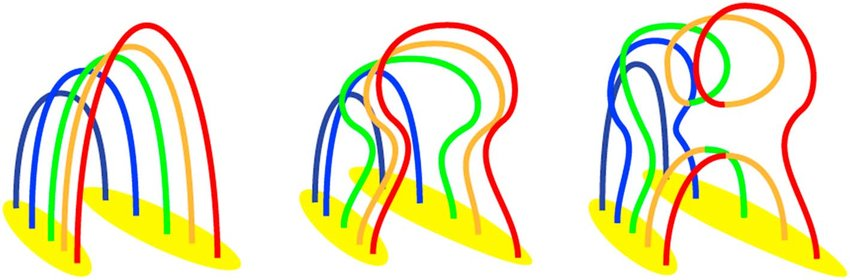
\includegraphics[width=0.9\textwidth]{standard_model.jpg}
\end{center}

$\to$ asymmetric \& unparallel ribbons (feet of $B$-lines) \\
$\to$ involve an inhomogeneous shear of the loops \\
$\to$ reconnection propagate along the arcade \\

\end{frame}



% ____________________________________________________________________________
\begin{frame}
\frametitle{Magnetic reconnection in planetary magnetosphere}

$\bullet$ Solar wind drives magnetosphere dynamics [\textit{Masters} 2018, GRL] : \\[0.4cm]

\begin{center}
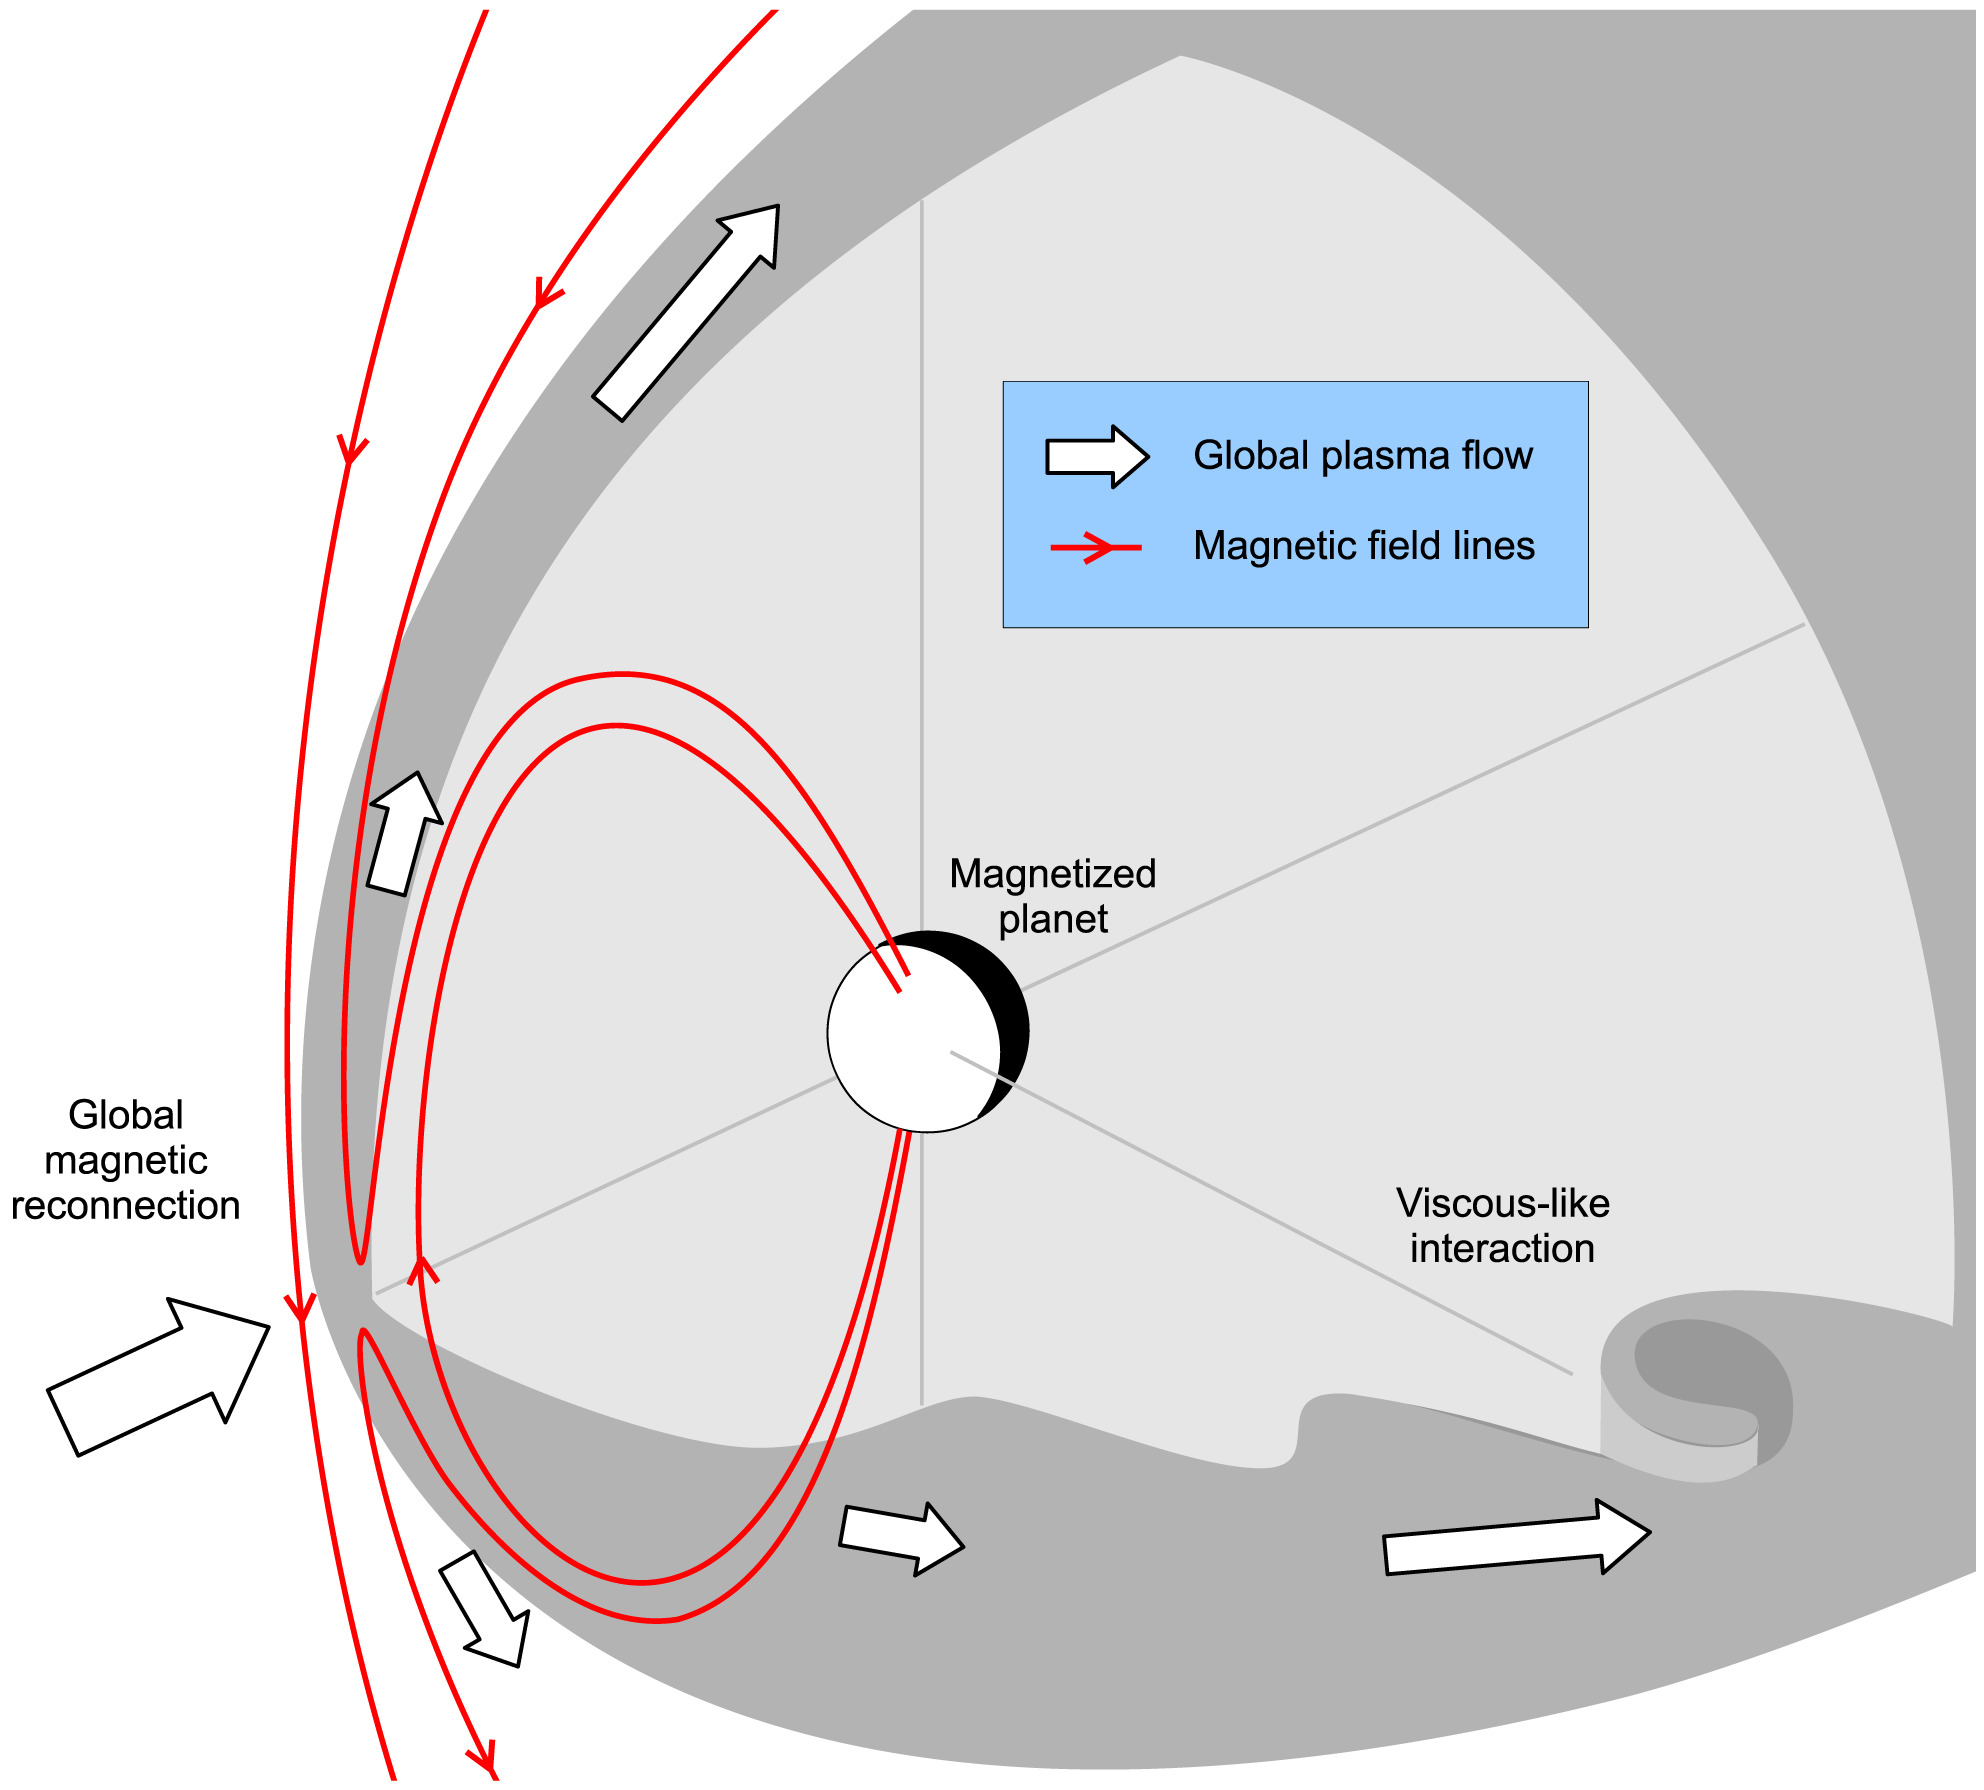
\includegraphics[width=0.5\textwidth]{magnetosphere_masters2018.jpg}
\end{center}

$\to$ magnetic reconnection spreads along a line \\
$\to$ thining of the current sheet driven by solar wind pressure \\
$\to$ viscous-like interaction (like KH instability) is secondary \\

\end{frame}





% ____________________________________________________________________________
\begin{frame}
\frametitle{Current sheets in plasma physics}

$\bullet$ Ubiquitous in the universe [\textit{Ji et al.} 2022, Nat. Rev. Phys.] : \\[0.4cm]

\begin{center}
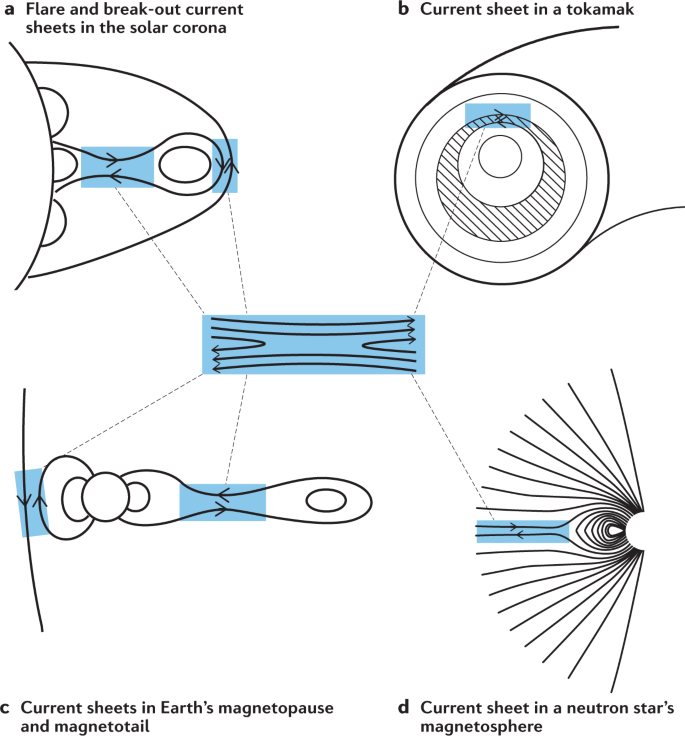
\includegraphics[width=0.5\textwidth]{current_sheet_ji2022.png}
\end{center}

$\to$ could be a PeVatron for cosmic rays, black-hole jets... \\

\end{frame}



%%% % ____________________________________________________________________________
%%% \begin{frame}
%%% \frametitle{Magnetic reconnection in 2D}
%%% 
%%% \begin{center}
%%% 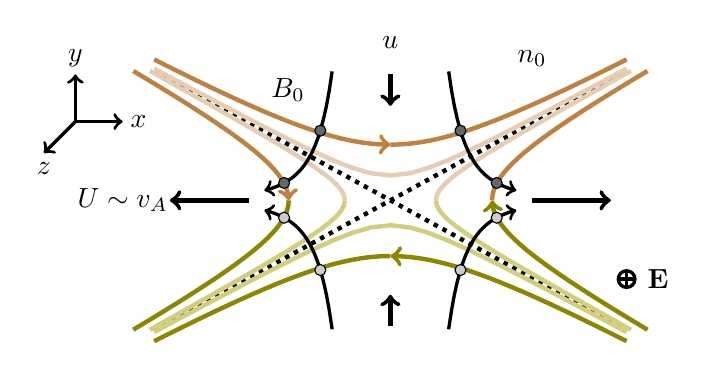
\begin{tikzpicture}[scale=1.0]

%\newcommand\XA{2} etc. and then \coordinate (A) at (\XA,\YA);

%\tikzset{declare function={f(\x)=\x;}}

\def\Xmin{-3.0}
\def\Xmax{+3.0}

\def\Ome{0.3}
\def\Lia{0.5}
\def\Lib{0.3}
\def\Lic{0.1}

\draw [domain=\Xmin: \Xmax, ultra thick, dotted] plot(\x,{-sqrt(\Ome)*\x});
\draw [domain=\Xmin: \Xmax, ultra thick, dotted] plot(\x,{ sqrt(\Ome)*\x});

\draw [domain=\Xmin: 0, ultra thick, draw=brown, ->] plot(\x,{sqrt( \Ome*\x*\x+\Lia)});
\draw [domain=0: \Xmax, ultra thick, draw=brown] plot(\x,{sqrt( \Ome*\x*\x+\Lia)});
\draw [domain=\Xmin: \Xmax, ultra thick, draw=brown!40] plot(\x,{sqrt( \Ome*\x*\x+\Lic)});

\draw [domain=\Xmin: 0, ultra thick, draw=olive] plot(\x,{-sqrt( \Ome*\x*\x+\Lia)});
\draw [domain=0: \Xmax, ultra thick, draw=olive, <-] plot(\x,{-sqrt( \Ome*\x*\x+\Lia)});
\draw [domain=\Xmin: \Xmax, ultra thick, draw=olive!40] plot(\x,{-sqrt( \Ome*\x*\x+\Lic)});

\draw [domain=\Xmin*sqrt(\Ome): 0, ultra thick, draw=olive, ->] plot({sqrt((\x*\x+\Lia)/\Ome)}, \x);
\draw [domain=0: \Xmax*sqrt(\Ome), ultra thick, draw=brown] plot({sqrt((\x*\x+\Lia)/\Ome)}, \x);
\draw [domain=\Xmin*sqrt(\Ome): 0, ultra thick, draw=olive!40] plot({sqrt((\x*\x+\Lic)/\Ome)}, \x);
\draw [domain=0: \Xmax*sqrt(\Ome), ultra thick, draw=brown!40] plot({sqrt((\x*\x+\Lic)/\Ome)}, \x);

\draw [domain=\Xmin*sqrt(\Ome): 0, ultra thick, draw=olive] plot({-sqrt((\x*\x+\Lia)/\Ome)}, \x);
\draw [domain=0: \Xmax*sqrt(\Ome), ultra thick, draw=brown, <-] plot({-sqrt((\x*\x+\Lia)/\Ome)}, \x);
\draw [domain=\Xmin*sqrt(\Ome): 0, ultra thick, draw=olive!40] plot({-sqrt((\x*\x+\Lic)/\Ome)}, \x);
\draw [domain=0: \Xmax*sqrt(\Ome), ultra thick, draw=brown!40] plot({-sqrt((\x*\x+\Lic)/\Ome)}, \x);

\def\KKK{0.6}
\def\XmiN{-1.6}
\def\XmaX{-0.74}

\draw [domain=\XmaX: \XmiN, very thick, ->] plot(\x, {\KKK*(-\x)^(-1/\Ome)});
\draw [domain=\XmaX: \XmiN, very thick, ->] plot(\x, {-\KKK*(-\x)^(-1/\Ome)});
\draw [domain=-\XmaX: -\XmiN, very thick, ->] plot(\x, {\KKK*(\x)^(-1/\Ome)});
\draw [domain=-\XmaX: -\XmiN, very thick, ->] plot(\x, {-\KKK*(\x)^(-1/\Ome)});


\def\Xa{0.89}
\def\Xb{1.35}

\filldraw[fill=black!60] (\Xa, {\KKK*(\Xa)^(-1/\Ome)}) circle (2pt);
\filldraw[fill=black!60] (\Xb, {\KKK*(\Xb)^(-1/\Ome)}) circle (2pt);
\filldraw[fill=black!60] (-\Xa, {\KKK*(\Xa)^(-1/\Ome)}) circle (2pt);
\filldraw[fill=black!60] (-\Xb, {\KKK*(\Xb)^(-1/\Ome)}) circle (2pt);

\filldraw[fill=black!20] (\Xa, -{\KKK*(\Xa)^(-1/\Ome)}) circle (2pt);
\filldraw[fill=black!20] (\Xb, -{\KKK*(\Xb)^(-1/\Ome)}) circle (2pt);
\filldraw[fill=black!20] (-\Xa, -{\KKK*(\Xa)^(-1/\Ome)}) circle (2pt);
\filldraw[fill=black!20] (-\Xb, -{\KKK*(\Xb)^(-1/\Ome)}) circle (2pt);



\draw[very thick] ( 3.0,-1.0) circle (3pt);
\draw[very thick] ( 2.9,-1.0) -- ( 3.1,-1.0);
\draw[very thick] ( 3.0,-1.1) -- ( 3.0,-0.9);
\node at ( 3.4,-1.0) {$\mathbf E$};

\draw[ultra thick, <-] (-2.8, 0) -- (-1.8, 0);
\draw[ultra thick, ->] (1.8, 0) -- (2.8, 0);
\node at (-3.4, 0.0) {$U \sim v_A$};

\draw[ultra thick, ->] ( 0.0, 1.6) -- ( 0.0, 1.2);
\draw[ultra thick, <-] ( 0.0,-1.2) -- ( 0.0,-1.6);
\node at ( 0.0, 2.0) {$u$};

\node at (-1.3, 1.4) {$B_0$};
\node at ( 1.8, 1.8) {$n_0$};


\draw[very thick, ->] (-4.0, 1.0) -- (-3.4, 1.0);
\node at (-3.2, 1.0) {$x$};
\draw[very thick, ->] (-4.0, 1.0) -- (-4.0, 1.6);
\node at (-4.0, 1.8) {$y$};
\draw[very thick, ->] (-4.0, 1.0) -- (-4.4, 0.6);
\node at (-4.4, 0.4) {$z$};


\end{tikzpicture}

%%% \end{center}
%%% 
%%% $\bullet$ Ohm's law : $\mathbf E = - \mathbf V \times \mathbf B - \frac{1}{en} [\mathbf j \times \mathbf B - \boldsymbol{\nabla} . \; \mathbf p_e] + \eta \mathbf j - \eta^{\prime} \Delta \mathbf j + m_e \D _t \mathbf j$ \\[0.4cm]
%%% $\bullet$ Efficiency  of reconnection measured by $E^{\prime} = E/B_0 v_A$ \\[0.4cm]
%%% $\to$ Dissipation $\equiv$ plasma resistivity : "slow reconnection" $E^{\prime} \le 0.01$\\
%%% $\to$ Dissipation $\equiv$ $e^-$ agyrotropy : "fast reconnection" $E^{\prime} \sim 0.1$ \\
%%% 
%%% \end{frame}
%%% 
%%% 
%%% 
% ____________________________________________________________________________
\begin{frame}
\frametitle{Big picture of 2D magnetic reconnection}

\begin{center}
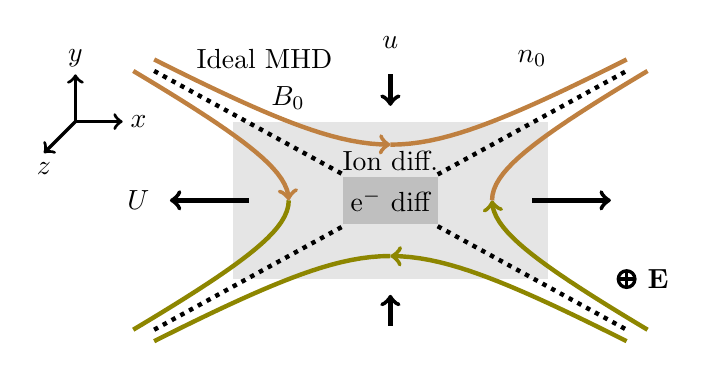
\begin{tikzpicture}[scale=1.0]

%\newcommand\XA{2} etc. and then \coordinate (A) at (\XA,\YA);

%\tikzset{declare function={f(\x)=\x;}}

\def\XIdiff{2.0}
\def\YIdiff{1.0}
\def\XEdiff{0.6}
\def\YEdiff{0.3}

\fill[gray!20] (-\XIdiff, -\YIdiff) rectangle (+\XIdiff, +\YIdiff);
\fill[gray!50] (-\XEdiff, -\YEdiff) rectangle (+\XEdiff, +\YEdiff);


\def\Xmin{-3.0}
\def\Xmax{+3.0}
\def\Xmed{+0.6}

\def\Ome{0.3}
\def\Lia{0.5}
\def\Lib{0.3}
\def\Lic{0.1}


\draw [domain=\Xmin: -\Xmed, ultra thick, dotted] plot(\x,{-sqrt(\Ome)*\x});
\draw [domain=\Xmed:  \Xmax, ultra thick, dotted] plot(\x,{-sqrt(\Ome)*\x});
\draw [domain=\Xmin: -\Xmed, ultra thick, dotted] plot(\x,{ sqrt(\Ome)*\x});
\draw [domain=\Xmed:  \Xmax, ultra thick, dotted] plot(\x,{ sqrt(\Ome)*\x});

\draw [domain=\Xmin: 0, ultra thick, draw=brown, ->] plot(\x,{sqrt( \Ome*\x*\x+\Lia)});
\draw [domain=0: \Xmax, ultra thick, draw=brown] plot(\x,{sqrt( \Ome*\x*\x+\Lia)});
%%% \draw [domain=\Xmin: \Xmax, ultra thick, draw=brown!40] plot(\x,{sqrt( \Ome*\x*\x+\Lic)});

\draw [domain=\Xmin: 0, ultra thick, draw=olive] plot(\x,{-sqrt( \Ome*\x*\x+\Lia)});
\draw [domain=0: \Xmax, ultra thick, draw=olive, <-] plot(\x,{-sqrt( \Ome*\x*\x+\Lia)});
%%% \draw [domain=\Xmin: \Xmax, ultra thick, draw=olive!40] plot(\x,{-sqrt( \Ome*\x*\x+\Lic)});

\draw [domain=\Xmin*sqrt(\Ome): 0, ultra thick, draw=olive, ->] plot({sqrt((\x*\x+\Lia)/\Ome)}, \x);
\draw [domain=0: \Xmax*sqrt(\Ome), ultra thick, draw=brown] plot({sqrt((\x*\x+\Lia)/\Ome)}, \x);
%%% \draw [domain=\Xmin*sqrt(\Ome): 0, ultra thick, draw=olive!40] plot({sqrt((\x*\x+\Lic)/\Ome)}, \x);
%%% \draw [domain=0: \Xmax*sqrt(\Ome), ultra thick, draw=brown!40] plot({sqrt((\x*\x+\Lic)/\Ome)}, \x);

\draw [domain=\Xmin*sqrt(\Ome): 0, ultra thick, draw=olive] plot({-sqrt((\x*\x+\Lia)/\Ome)}, \x);
\draw [domain=0: \Xmax*sqrt(\Ome), ultra thick, draw=brown, <-] plot({-sqrt((\x*\x+\Lia)/\Ome)}, \x);
%%% \draw [domain=\Xmin*sqrt(\Ome): 0, ultra thick, draw=olive!40] plot({-sqrt((\x*\x+\Lic)/\Ome)}, \x);
%%% \draw [domain=0: \Xmax*sqrt(\Ome), ultra thick, draw=brown!40] plot({-sqrt((\x*\x+\Lic)/\Ome)}, \x);

%%% \def\KKK{0.6}
%%% \def\XmiN{-1.6}
%%% \def\XmaX{-0.74}
%%% 
%%% \draw [domain=\XmaX: \XmiN, very thick, ->] plot(\x, {\KKK*(-\x)^(-1/\Ome)});
%%% \draw [domain=\XmaX: \XmiN, very thick, ->] plot(\x, {-\KKK*(-\x)^(-1/\Ome)});
%%% \draw [domain=-\XmaX: -\XmiN, very thick, ->] plot(\x, {\KKK*(\x)^(-1/\Ome)});
%%% \draw [domain=-\XmaX: -\XmiN, very thick, ->] plot(\x, {-\KKK*(\x)^(-1/\Ome)});


%%% \def\Xa{0.89}
%%% \def\Xb{1.35}
%%% 
%%% \filldraw[fill=black!60] (\Xa, {\KKK*(\Xa)^(-1/\Ome)}) circle (2pt);
%%% \filldraw[fill=black!60] (\Xb, {\KKK*(\Xb)^(-1/\Ome)}) circle (2pt);
%%% \filldraw[fill=black!60] (-\Xa, {\KKK*(\Xa)^(-1/\Ome)}) circle (2pt);
%%% \filldraw[fill=black!60] (-\Xb, {\KKK*(\Xb)^(-1/\Ome)}) circle (2pt);
%%% 
%%% \filldraw[fill=black!20] (\Xa, -{\KKK*(\Xa)^(-1/\Ome)}) circle (2pt);
%%% \filldraw[fill=black!20] (\Xb, -{\KKK*(\Xb)^(-1/\Ome)}) circle (2pt);
%%% \filldraw[fill=black!20] (-\Xa, -{\KKK*(\Xa)^(-1/\Ome)}) circle (2pt);
%%% \filldraw[fill=black!20] (-\Xb, -{\KKK*(\Xb)^(-1/\Ome)}) circle (2pt);



\draw[very thick] ( 3.0,-1.0) circle (3pt);
\draw[very thick] ( 2.9,-1.0) -- ( 3.1,-1.0);
\draw[very thick] ( 3.0,-1.1) -- ( 3.0,-0.9);
\node at ( 3.4,-1.0) {$\mathbf E$};

\draw[ultra thick, <-] (-2.8, 0) -- (-1.8, 0);
\draw[ultra thick, ->] (1.8, 0) -- (2.8, 0);
\node at (-3.2, 0.0) {$U$};

\draw[ultra thick, ->] ( 0.0, 1.6) -- ( 0.0, 1.2);
\draw[ultra thick, <-] ( 0.0,-1.2) -- ( 0.0,-1.6);
\node at ( 0.0, 2.0) {$u$};

\node at (-1.3, 1.3) {$B_0$};
\node at ( 1.8, 1.8) {$n_0$};

\node at (-1.6, 1.8) {Ideal MHD};
\node at (-0.0, 0.5) {Ion diff.};
\node at (-0.0, 0.0) {e$^-$ diff};


\draw[very thick, ->] (-4.0, 1.0) -- (-3.4, 1.0);
\node at (-3.2, 1.0) {$x$};
\draw[very thick, ->] (-4.0, 1.0) -- (-4.0, 1.6);
\node at (-4.0, 1.8) {$y$};
\draw[very thick, ->] (-4.0, 1.0) -- (-4.4, 0.6);
\node at (-4.4, 0.4) {$z$};


\end{tikzpicture}

\end{center}

$\bullet$ Ohm's law : $\displaystyle \mathbf E = - \mathbf V \times \mathbf B - \frac{1}{en} [\mathbf j \times \mathbf B - \boldsymbol{\nabla} . \; \mathbf p_e] + \eta \mathbf j - \eta^{\prime} \Delta \mathbf j + m_e \D _t \mathbf j$ \\[0.2cm]
$\bullet$ Efficiency  of reconnection measured by $E^{\prime} = E/B_0 v_A$ \\[0.1cm]
$\to$ Ideal term in the MHD region \\
$\to$ Hall term in the Ion diffusion region (control $E^{\prime}$) \\
$\to$ Agyrotropic pressure term in the electron region (control $J_z$) \\

\end{frame}



% ____________________________________________________________________________
\begin{frame}
\frametitle{Pending questions}

$\bullet$ What is the origin of the local dissipation? \\[0.3cm]
$\bullet$ What is the importance of the 3D geometry? \\[0.3cm]
$\bullet$ How efficiently plasma and $B$-field are transported through the reconnection site? \\[0.3cm]
$\bullet$ How and where do X lines form in the current sheet? \\[0.3cm]
$\bullet$ X line formation: local spreading in a global context? \\[0.3cm]
$\bullet$ What controls their length? \\[0.3cm]
$\bullet$ How do they respond to the temporal variations of external conditions? \\[0.3cm]
$\bullet$ What are the respective roles of large scale inhomogeneities and local kinetic effects? \\[0.3cm]

\end{frame}



% ____________________________________________________________________________
\begin{frame}
\frametitle{Magnetized plasma loop using a ns-laser}

$\bullet$ Plasma produced by a ns-laser on a solid target \\
$\bullet$ $B$-field produced by Biermann-battery effect

\begin{center}
\colorlet{mylightgray}{black!30}
\colorlet{mydarkgray}{black!50}

\colorlet{mydarkblue}{blue!50!black}
\colorlet{watercol}{blue!80!cyan!10!white}
\colorlet{darkwatercol}{blue!80!cyan!20!white}

\tikzstyle{plasma}=[very thick, draw=black, top color=mydarkgray, bottom color=mydarkgray]

\tikzstyle{water}=[draw=mydarkblue,top color=watercol!90,bottom color=watercol!90!black,shading angle=5]
\tikzstyle{vertical water}=[water, top color=watercol!90!black!90,bottom color=watercol!90!black!90,middle color=watercol!80,shading angle=90]
\tikzstyle{dark water}=[draw=mydarkblue,top color=darkwatercol,bottom color=darkwatercol!80!black,shading angle=5]


\begin{tikzpicture}[scale=0.4]
  \def\Rx{5.0}      % tank horizontal radius
  \def\Ry{3.0}      % tank vertical radius
  \def\rx{0.5*\Rx} % column horizontal radius
  \def\ry{0.5*\Ry} % column vertical radius
  \def\H{1.5}       % height tank
  \def\h{0.94*\H}   % height water
  \def\l{-0.7*\H}   % height water
  \def\y{0.40*\H}   % vertical position piece
  \def\dy{0.10*\H}  % height piece
  \def\shif{0.6}

  \draw[very thick, fill=mylightgray] (-\Rx,\h) -- (-\Rx,0) arc (180:360:{\Rx} and {\Ry}) -- (\Rx,\h);
  %\draw[very thick, dotted] (-\Rx,0) -- (-\Rx,\l) arc (180:360:{\Rx} and {\Ry}) -- (\Rx,0);
  \draw[fill=mydarkgray, very thick] (0,\h) ellipse ({\Rx} and {\Ry});
  \draw[ultra thick, fill=white] (0,\h) ellipse ({\rx} and {\ry});
  \draw[very thick, dotted, color=brown] (-\Rx,0) -- (-\Rx,\l);
  \draw[very thick, dotted, color=brown] ( \Rx,0) -- ( \Rx,\l);
  \draw[very thick, dashed, color=brown] (0,\l) ellipse ({\Rx} and {\Ry});
  \node[color=brown] at (5.0,-4.0) {solid target};
  \draw[<-, ultra thick] (0+\rx, \h) arc [start angle=0, end angle=60, x radius ={\rx}, y radius={\ry}];
  \draw[ultra thick] (0,\h) ellipse ({\Rx} and {\Ry});
  \draw[<-, ultra thick] (0+\Rx, \h) arc [start angle=0, end angle=60, x radius ={\Rx}, y radius={\Ry}];

  \draw[ultra thick, ->, color=olive] (0, 5*\H) -- (0, 0);
  \node[color=olive] at (0.0, 8.0) {ns-laser};

  \draw[ultra thick, ->] (\shif, 4.6*\H) -- (\shif, 3.8*\H);
  \node at (1.7, 6.3) {$\boldsymbol{\nabla} n_e$};
  \draw[ultra thick, ->] (-4.8, \h) -- (-3.4, \h);
  \draw[ultra thick, ->] (0, -1.4) -- (0, -0.4);
  \node at (-1.0, -1.0) {$\boldsymbol{\nabla} T_e$};


  %%% % COLUMN + PIECE
  %%% \draw[dark water]
  %%%   (-\rx,\y) -- (-\rx,\y-\dy) arc (180:360:{\rx} and {\ry}) -- (\rx,\y);
  %%% \draw[dark water]
  %%%   (0,\y) ellipse ({\rx} and {\ry});
  %%% \draw[dark water,opacity=0.50,draw=none] % column
  %%%   (-\rx,\h) -- (-\rx,\y) arc (180:360:{\rx} and {\ry}) -- (\rx,\h) arc(360:180:{\rx} and {\ry}) -- cycle;
  %%% \draw[blue!20!black,dashed,very thin,opacity=0.50] (-\rx,\y) -- (-\rx,\h) (\rx,\y) -- (\rx,\h);
  %%% \draw[dark water,opacity=0.50] % top column
  %%%   (0,\h) ellipse ({\rx} and {\ry});
  %%% \draw[blue!30!black]
  %%%   (0,\h) ellipse ({\Rx} and {\Ry});
  %%% 
  %%% % CONTAINER
  %%% \draw[thick]
  %%%   (-\Rx,\H) -- (-\Rx,0) arc (180:360:{\Rx} and {\Ry}) -- (\Rx,\H);
  %%% \draw[thick]
  %%%   (0,\H) ellipse ({\Rx} and {\Ry});
  %%% 
  %%% % LABELS
  %%% \node[scale=0.98] at ({-0.45*(\Rx+\rx)},1.04*\h) {$P_\mathrm{atm}$}; %{\contour{watercol}{$P_\mathrm{atm}$}};
  %%% \node at ({-0.40*(\Rx+\rx)},{\y-0.5*\dy}) {$P$};
  %%% \node[above=-2] at (0,\y+\ry) {$A$};
  %%% \draw[<->] (1.2*\Rx,\y) --++ (0,\h-\y) node[midway,fill=white,inner sep=1] {$h$};
  
\end{tikzpicture}


\end{center}

$\Rightarrow$ The B-field produced on \underline{front face} is clock-wise oriented :
$$
\partial_t \mathbf B = - \frac{1}{en_e} \boldsymbol{\nabla} n_e \times \boldsymbol{\nabla} T_e
$$

\end{frame}



% ____________________________________________________________________________
\begin{frame}
\frametitle{Reconnection between 2 magnetized plasma loops}

$\bullet$ Distance between the 2 focal spots $\geq$ twice the plume radii

\begin{center}
\colorlet{mylightgray}{black!30}
\colorlet{mydarkgray}{black!50}


\begin{tikzpicture}[scale=0.4]
  \def\Rx{4.0}      % tank horizontal radius
  \def\Ry{3.0}      % tank vertical radius
  \def\rx{0.5*\Rx} % column horizontal radius
  \def\ry{0.5*\Ry} % column vertical radius
  \def\H{1.5}       % height tank
  \def\h{0.94*\H}   % height water
  \def\zob{9.0}   % height water

  \draw[very thick, fill=mylightgray] (-\Rx,\h) -- (-\Rx,0) arc (180:360:{\Rx} and {\Ry}) -- (\Rx,\h);
  \draw[very thick, fill=mylightgray] (\zob-\Rx,\h) -- (\zob-\Rx,0) arc (180:360:{\Rx} and {\Ry}) -- (\zob+\Rx,\h);

  \draw[fill=mydarkgray, very thick] (0,\h) ellipse ({\Rx} and {\Ry});
  \draw[fill=mydarkgray, very thick] (\zob,\h) ellipse ({\Rx} and {\Ry});

  \draw[ultra thick, fill=white] (0,\h) ellipse ({\rx} and {\ry});
  \draw[ultra thick] (0,\h) ellipse ({\Rx} and {\Ry});

  \draw[ultra thick, fill=white] (\zob,\h) ellipse ({\rx} and {\ry});
  \draw[ultra thick] (\zob,\h) ellipse ({\Rx} and {\Ry});

  \draw[<-, ultra thick] (0+\rx, \h) arc [start angle=0, end angle=60, x radius ={\rx}, y radius={\ry}];
  \draw[<-, ultra thick] (0+\Rx, \h) arc [start angle=0, end angle=60, x radius ={\Rx}, y radius={\Ry}];

  \draw[<-, ultra thick] (\zob-\rx, \h) arc [start angle=180, end angle=210, x radius ={\rx}, y radius={\ry}];
  \draw[<-, ultra thick] (\zob-\Rx, \h) arc [start angle=180, end angle=210, x radius ={\Rx}, y radius={\Ry}];

  \draw[ultra thick, ->] (-3.6, 4.0) -- (-2.8, 5.0);
  \node at (-2.7, 5.4) {$x$};
  \draw[ultra thick, ->] (-3.6, 4.0) -- (-5.0, 4.0);
  \node at (-5.3, 4.0) {$y$};
  \draw[ultra thick, ->] (-3.6, 4.0) -- (-3.6, 5.6);
  \node at (-3.6, 5.9) {$z$};


\end{tikzpicture}


\end{center}

$\bullet$ The current sheet is building up during the irradiation \\
$\bullet$ Lundqvist number $S \sim 10^3$ (with Spitzer-Harm resistivity) \\
$\to$ aspect ratio of the current sheet $L/\delta < $ 50 \\
$\to$ we then are \underline{not in the plasmoid regime} \\
$\bullet$ Curvature of the B-field in favour of single X-type reconnection \\
$\bullet$ Numerical approach with a 2D Hybrid-PIC code \\

\end{frame}



% ____________________________________________________________________________
\begin{frame}
\frametitle{Lasers configurations (first shot - 2019) on LMJ}

\begin{center}
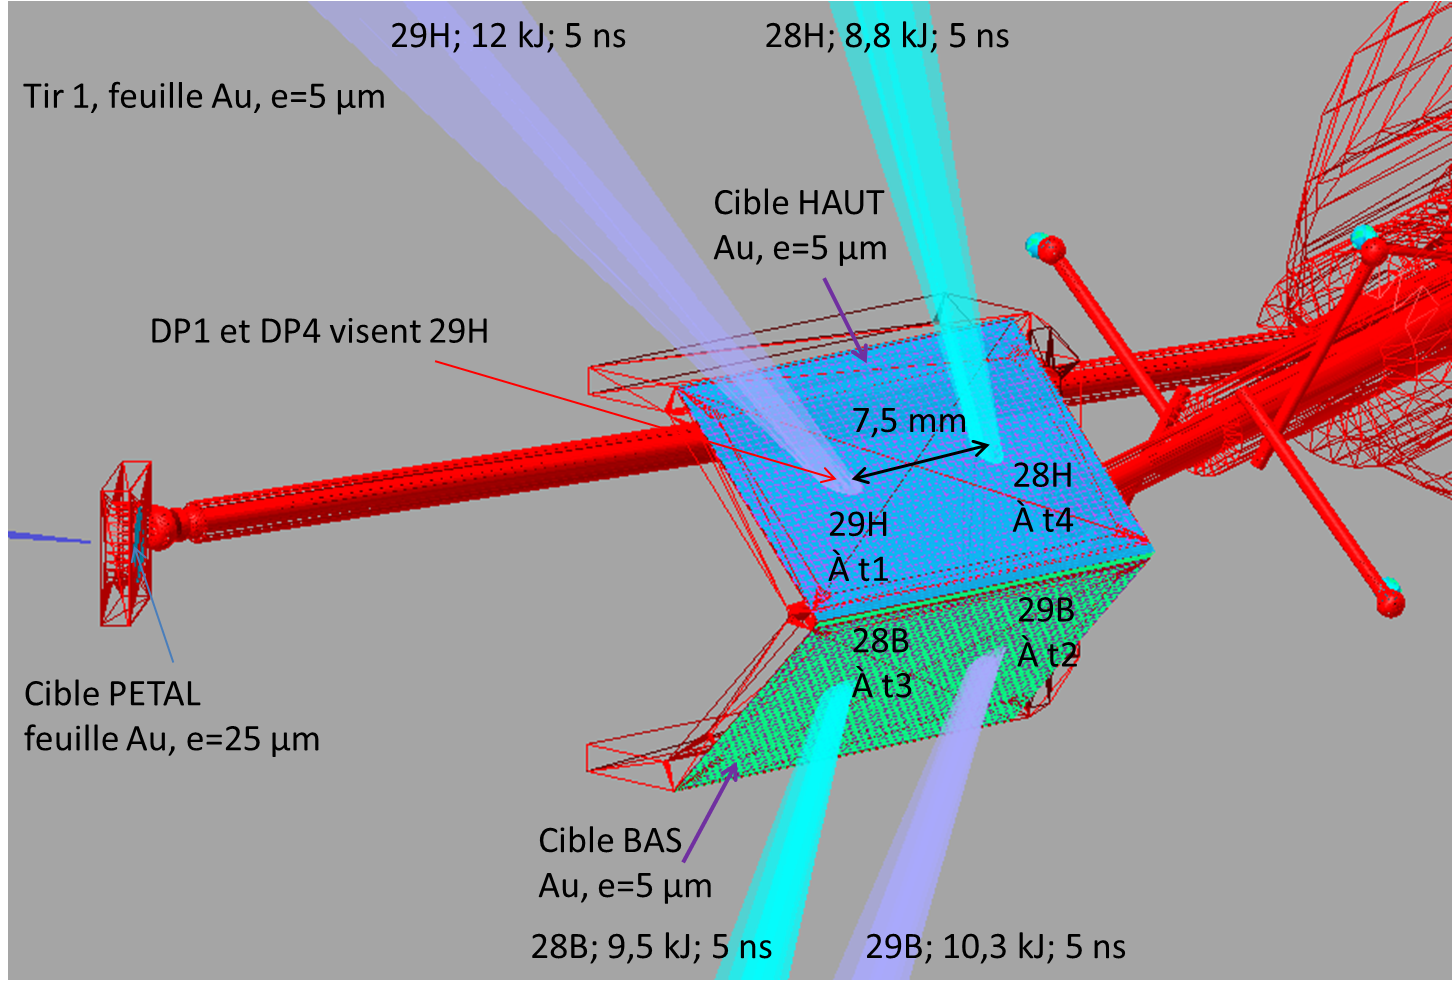
\includegraphics[width=0.9\textwidth]{tir1.png}
\end{center}

\end{frame}



% ____________________________________________________________________________
\begin{frame}
\frametitle{Lasers parameters}

\begin{center}
\begin{tabular}{lll}
\hline
\hline
\hspace{1.0cm} & LMJ\hspace{2.0cm}  & PETAL\hspace{1.0cm}  \\
\hline
Pulse duration             & 5 ns                    & 0.7 ps \\
Energy                     & 12 kJ                   & 400 J \\
Solid target               & \texttt{Au} - 5 $\mu$m  & \texttt{Au} - 25 $\mu$m \\
Wave length                & 351 nm                  & 1053 nm \\
\hline
\hline
\end{tabular}
\end{center}

\bigskip

$\bullet$ we used 6 quads : C28, C29, C10, both H \& B \\
$\bullet$ laser incidence depends on the quad for experimental reasons  \\
$\to$ energy is then modulated for somewhat similar plasma loops \\
$\bullet$ proton probe incidence of 34$^o$ \\
$\bullet$ hot spots separation : 7.5 mm \& 1.5 mm for reconnection \\
$\bullet$ a total of 7 shots (1 on \texttt{Ti}-foil) \\
$\bullet$ 3 times for 2-loops and 3-loops reconnection : 2.1, 3.2 \& 4.3 ns \\

\end{frame}



% ____________________________________________________________________________
\begin{frame}
\frametitle{Plasmas parameters}

$\bullet$ From \texttt{fci2} simulation (for a 1-plume plasma) :

\begin{center}
\begin{tabular}{lll}
\hline
\hline
& Plasma plume & Proton beam \hspace{2.0cm}\\
\hline
Magnetic field             & $\sim$ 600 nT                              & \\
Electron density           & $\sim$ 4 $\times$ 10$^{27}$ m$^{-3}$       & \\
Mean flow                  & $\sim 2 \times 10^5$ m.s$^{-1}$            & $\sim c$ \\
Kinetic energy             & $\sim$ 100 eV                              & $\sim$ 42 MeV \\
$\beta$ parameter          & $\beta_e = 0.5$, $\beta_i = 0.02$          & \\
Loop radii                 & $\sim$ 300 $\to$ 900 $\mu$m                & \\
Ion Inertial length        & $\sim$ 4 $\mu$m                            & \\
Ion Gyroperiod             & $\sim$ 17 ps                               & \\
Alfvén velocity            & $\sim 2 \times 10^5$ m.s$^{-1}$            & \\
\hline
\hline
\end{tabular}
\end{center}

$\to$ close to the $\beta \sim 1$ regime \\
$\to$ magnetization parameter $\sigma \ll 1$ \\

\end{frame}



%%% % ____________________________________________________________________________
%%% \begin{frame}
%%% \frametitle{Reconnection between 3 magnetized plasma loops}
%%% 
%%% $\bullet$ Why did we also used 3-plumes reconnection ?
%%% \begin{center}
%%% \colorlet{mylightgray}{black!30}
\colorlet{mydarkgray}{black!50}


\begin{tikzpicture}[scale=0.4]
  \def\Rx{4.0}      % tank horizontal radius
  \def\Ry{3.0}      % tank vertical radius
  \def\rx{0.5*\Rx} % column horizontal radius
  \def\ry{0.5*\Ry} % column vertical radius
  \def\H{1.5}       % height tank
  \def\h{0.94*\H}   % height water
  \def\xdeux{9.0}   % height water
  \def\xtrois{0.5*\xdeux}   % height water
  \def\yyy{6.0}   % height water

  \draw[very thick, fill=mylightgray] (-\Rx,\h) -- (-\Rx,0) arc (180:360:{\Rx} and {\Ry}) -- (\Rx,\h);
  \draw[very thick, fill=mylightgray] (\xdeux-\Rx,\h) -- (\xdeux-\Rx,0) arc (180:360:{\Rx} and {\Ry}) -- (\xdeux+\Rx,\h);
  \draw[very thick, fill=mylightgray] (\xtrois-\Rx,\yyy+\h) -- (\xtrois-\Rx,\yyy+0) arc (180:360:{\Rx} and {\Ry}) -- (\xtrois+\Rx,\yyy+\h);

  \draw[fill=mydarkgray, very thick] (0,\h) ellipse ({\Rx} and {\Ry});
  \draw[fill=mydarkgray, very thick] (\xdeux,\h) ellipse ({\Rx} and {\Ry});
  \draw[fill=mydarkgray, very thick] (\xtrois,\yyy+\h) ellipse ({\Rx} and {\Ry});

  \draw[ultra thick, fill=white] (0,\h) ellipse ({\rx} and {\ry});
  \draw[ultra thick] (0,\h) ellipse ({\Rx} and {\Ry});

  \draw[ultra thick, fill=white] (\xdeux,\h) ellipse ({\rx} and {\ry});
  \draw[ultra thick] (\xdeux,\h) ellipse ({\Rx} and {\Ry});

  \draw[ultra thick, fill=white] (\xtrois,\yyy+\h) ellipse ({\rx} and {\ry});
  \draw[ultra thick] (\xtrois,\yyy+\h) ellipse ({\Rx} and {\Ry});

  \draw[<-, ultra thick] (0+\rx, \h) arc [start angle=0, end angle=60, x radius ={\rx}, y radius={\ry}];
  \draw[<-, ultra thick] (0+\Rx, \h) arc [start angle=0, end angle=60, x radius ={\Rx}, y radius={\Ry}];

  \draw[<-, ultra thick] (\xdeux-\rx, \h) arc [start angle=180, end angle=210, x radius ={\rx}, y radius={\ry}];
  \draw[<-, ultra thick] (\xdeux-\Rx, \h) arc [start angle=180, end angle=210, x radius ={\Rx}, y radius={\Ry}];

  \draw[<-, ultra thick] (\xtrois, \yyy-1.13*\h+\ry) arc [start angle=270, end angle=300, x radius ={\rx}, y radius={\ry}];
  \draw[<-, ultra thick] (\xtrois, \yyy-1.13*\h) arc [start angle=270, end angle=300, x radius ={\Rx}, y radius={\Ry}];

  \draw[ultra thick, ->] (-3.6, 4.0) -- (-2.8, 5.0);
  \node at (-2.7, 5.4) {$x$};
  \draw[ultra thick, ->] (-3.6, 4.0) -- (-5.0, 4.0);
  \node at (-5.3, 4.0) {$y$};
  \draw[ultra thick, ->] (-3.6, 4.0) -- (-3.6, 5.6);
  \node at (-3.6, 5.9) {$z$};


\end{tikzpicture}


%%% \end{center}
%%% 
%%% $\bullet$ The plasma outflow (ejecta) is "trapped" in closed structures \\
%%% $\bullet$ Creation of a closed magnetic structure \\
%%% $\to$ being quite small, should be "quite planar"
%%% 
%%% \end{frame}
%%% 
%%% 
%%% 



% ____________________________________________________________________________
\begin{frame}
\frametitle{Diagnostics (LMJ experiments in 2019)}

$\bullet$ Proton radiography using PETAL on a solid target \\
$\to$ a proton beam is created with ps-laser on solid target by TNSA \\
$\to$ collected on a stack of Radio-Chromic-Films (resolved in energy) \\
$\to$ the proton dose give insights on the path-integrated $B$-field \\

\bigskip
\bigskip

$\bullet$ DMX \\
$\to$ integrated spectra (arbitrary units) depending on time \\

\bigskip
\bigskip

$\bullet$ DP1 \& DP4 \\
$\to$ provides an image of the focal spot \\

%%% \bigskip
%%% \bigskip
%%% 
%%% $\Rightarrow$ Thomson parabola could be nice: $n_e$, $V_i$, $T_e$, $T_i$ \\

\end{frame}



% ____________________________________________________________________________
\begin{frame}
\frametitle{B-field pictured by proton-radiography}

$\bullet$ Proton beam (42 MeV max. energy) produced by TNSA \\
$\to$ using PETAL on a 25 $\mu$m gold foil

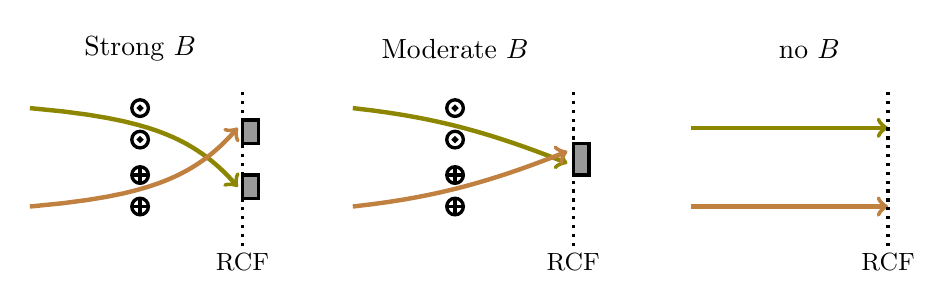
\begin{tikzpicture}[scale=0.5]

\definecolor{mycolor}{rgb}{0,0.6,0.5}

\def\asympL{+2.8}
\def\asympM{+1.8}
\def\shiftone{+7.0}

\tikzset{declare function={trajL(\x)=(-0.4*\x-4)+\asympL/(\x-1);}}
\tikzset{declare function={trajM(\x)=(-2.0*\x-4)+\asympM/(\x-1);}}
\tikzset{declare function={chameau(\x)=-4.4+exp(-5.0*(\x-2)*(\x-2))+exp(-5.0*(\x-0)*(\x-0));}}
\tikzset{declare function={dromadaire(\x)=+1.4+exp(-2.0*(\x-1)*(\x-1));}}

\node at (-7.0 ,2.0) {Strong $B$};

\draw [domain=-1.5:+0.5, ultra thick, olive, <-] plot({trajL(\x)}, \x);
\draw [domain=-1.5:+0.5, ultra thick, brown, <-] plot({trajL(\x)}, (-1.5-\x);

\draw[very thick] (-7.0,-0.3) circle (6pt);
\draw[very thick] (-7.0,-0.3) circle (1pt);
\draw[very thick] (-7.0, 0.5) circle (6pt);
\draw[very thick] (-7.0, 0.5) circle (1pt);

\draw[very thick] (-7.0,-1.2) circle (6pt);
\draw[very thick] (-7.2,-1.2) -- (-6.8,-1.2);
\draw[very thick] (-7.0,-1.4) -- (-7.0,-1.0);
\draw[very thick] (-7.0,-2.0) circle (6pt);
\draw[very thick] (-7.2,-2.0) -- (-6.8,-2.0);
\draw[very thick] (-7.0,-2.2) -- (-7.0,-1.8);

\draw[dotted, very thick] (-4.4,-3.0) -- (-4.4,+1.0);

\node at (-4.4,-3.4) {{\small RCF}};

\draw[fill=black!40, very thick] ( -4.4, -1.8) -- (-4.4, -1.2) -- (-4.0, -1.2) -- (-4.0, -1.8) -- cycle;
\draw[fill=black!40, very thick] ( -4.4, -0.4) -- (-4.4, +0.2) -- (-4.0, +0.2) -- (-4.0, -0.4) -- cycle;

%\draw [domain=-3.0:+3.0, line width=0.1cm, cyan] plot(\x, {\exp(-\x)});
%\addplot {\gauss(1,0.75)};
%\draw[cyan] plot[id=f7,domain=-4.25:4.25,samples=100] function {10*exp(-x*x/2)};
%\filldraw [fill=red] plot[id=f6,domain=-20:30] function {exp(-x*x/2)} -- (3,0)  -- (2,0) -- cycle;
%\filldraw [domain=-2.0:+3.0, rotate=-90, olive] plot(\x, {chameau(\x)});



\node at ( 1.0 ,2.0) {Moderate $B$};

\draw [domain=-0.9:+0.5, ultra thick, olive, <-] plot({\shiftone+trajM(\x)}, \x);
\draw [domain=-0.9:+0.5, ultra thick, brown, <-] plot({\shiftone+trajM(\x)}, (-1.5-\x);

\draw[very thick] ( 1.0,-0.3) circle (6pt);
\draw[very thick] ( 1.0,-0.3) circle (1pt);
\draw[very thick] ( 1.0, 0.5) circle (6pt);
\draw[very thick] ( 1.0, 0.5) circle (1pt);

\draw[very thick] ( 1.0,-1.2) circle (6pt);
\draw[very thick] ( 0.8,-1.2) -- ( 1.2,-1.2);
\draw[very thick] ( 1.0,-1.4) -- ( 1.0,-1.0);
\draw[very thick] ( 1.0,-2.0) circle (6pt);
\draw[very thick] ( 0.8,-2.0) -- ( 1.2,-2.0);
\draw[very thick] ( 1.0,-2.2) -- ( 1.0,-1.8);

\draw[dotted, very thick] (+4.0,-3.0) -- (+4.0,+1.0);

\node at ( 4.0,-3.4) {{\small RCF}};

\draw[fill=black!40, very thick] (4.0, -1.2) -- (4.0, -0.4) -- (4.4, -0.4) -- (4.4, -1.2) -- cycle;

%\filldraw [domain=-3.0:+3.0, rotate=-90, olive] plot(\x, {dromadaire(\x)});



\node at ( 10.0 ,2.0) {no $B$};

\draw [domain=+7.0:+12.0, ultra thick, olive, ->] plot(\x, +0.0);
\draw [domain=+7.0:+12.0, ultra thick, brown, ->] plot(\x, -2.0);

\draw[dotted, very thick] (+12.0,-3.0) -- (+12.0,+1.0);

\node at ( 12.0,-3.4) {{\small RCF}};

\end{tikzpicture}


$\bullet$ Strong $B$ $\Rightarrow$ before Reconnection : "open mouth" \\
$\bullet$ Moderate $B$ $\Rightarrow$ during reconnection : "closed mouth" \\
$\bullet$ no $B$ $\Rightarrow$ after reconnection : nothing ! \\

\end{frame}



% ____________________________________________________________________________
\begin{frame}
\frametitle{Synthetic RCF for 10 MeV proton beam}

\begin{center}
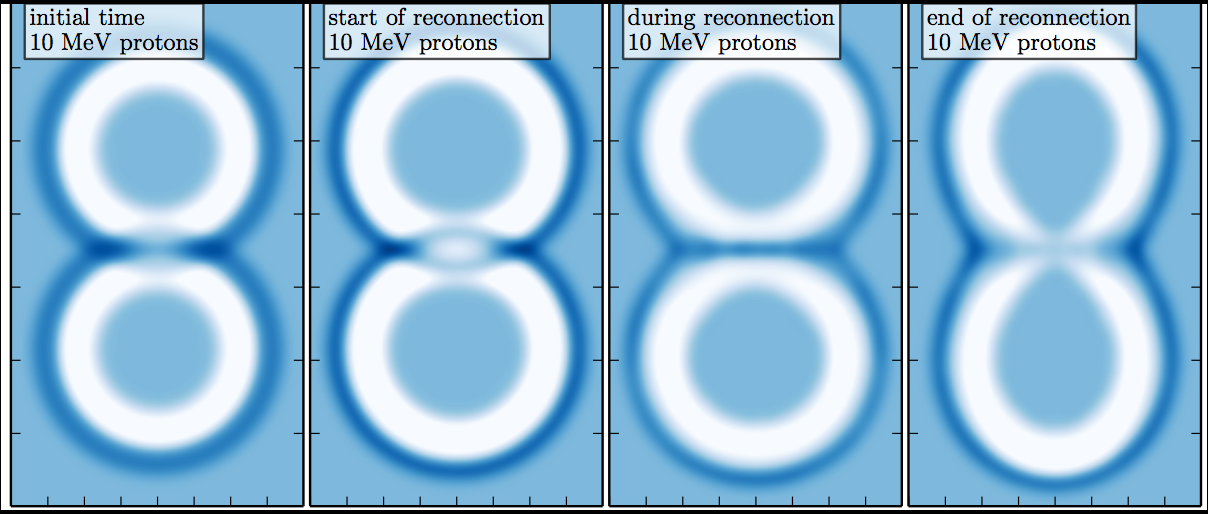
\includegraphics[width=0.8\textwidth]{rcf2D.png}
\end{center}

$\to$ a "mouth" open when B field is compressed\\
$\to$ but closes when reconnection operates (and decrease B)\\

\end{frame}



% ____________________________________________________________________________
\begin{frame}
\frametitle{Proton radiographies from LMJ 2019 experiment}

\begin{center}
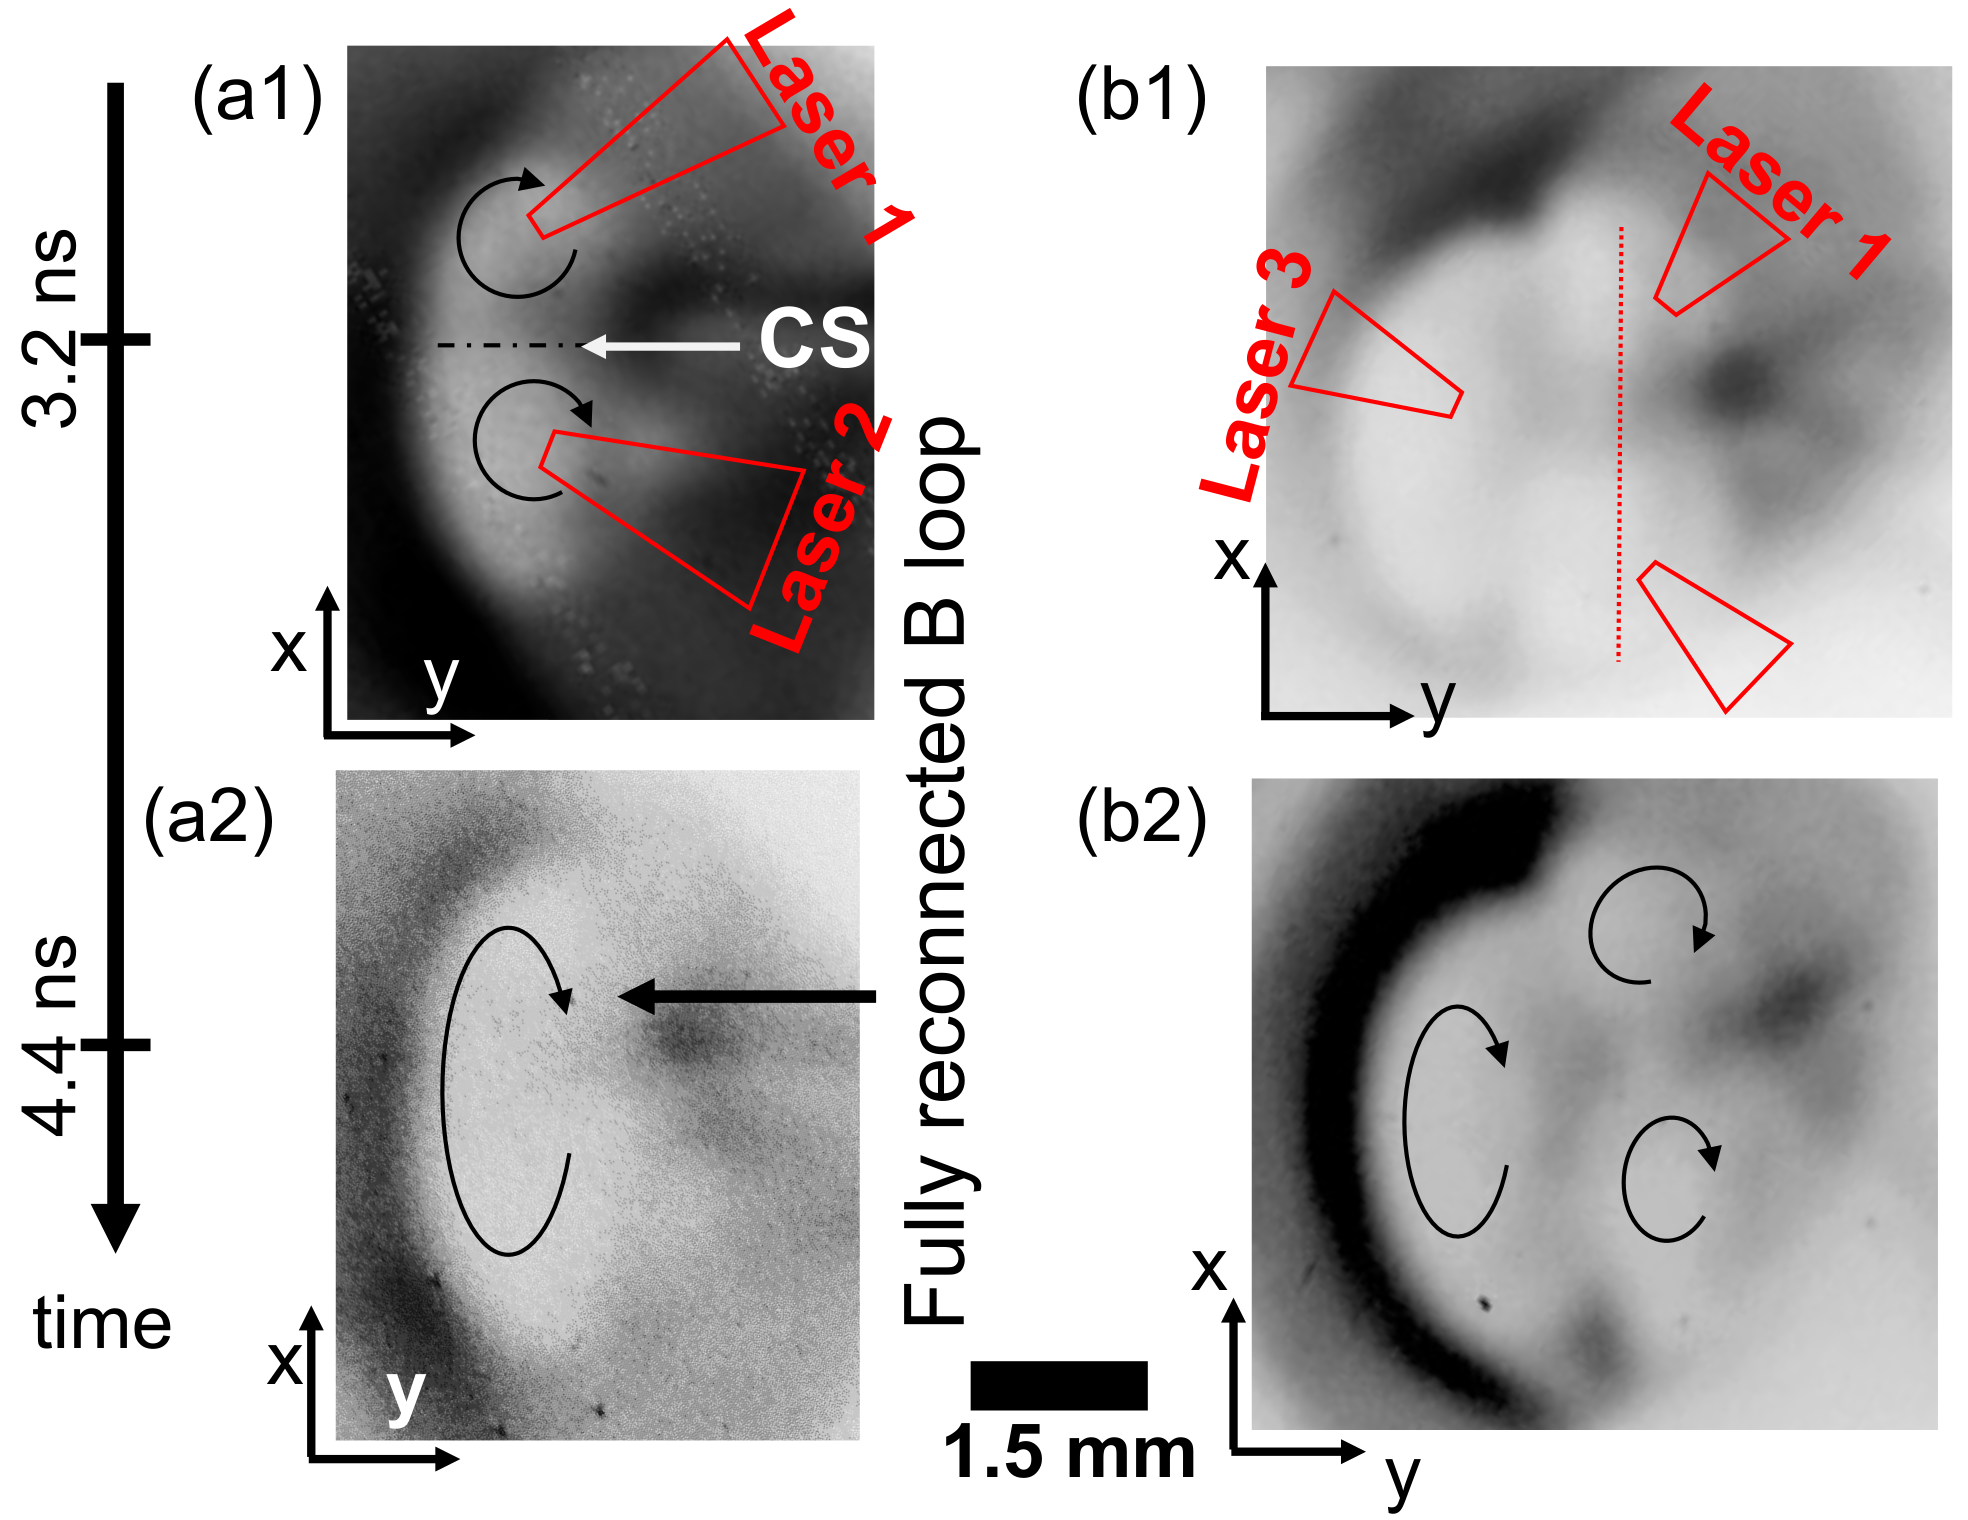
\includegraphics[width=0.8\textwidth]{rcf_lmj.png}
\end{center}

\end{frame}



% ____________________________________________________________________________
\begin{frame}
\frametitle{B-field reconstruction using \texttt{problem} solver}

$\bullet$ Maxwell-Faraday : relation between magnetic flux $\partial_t \phi$ and $E$ \\

\begin{center}
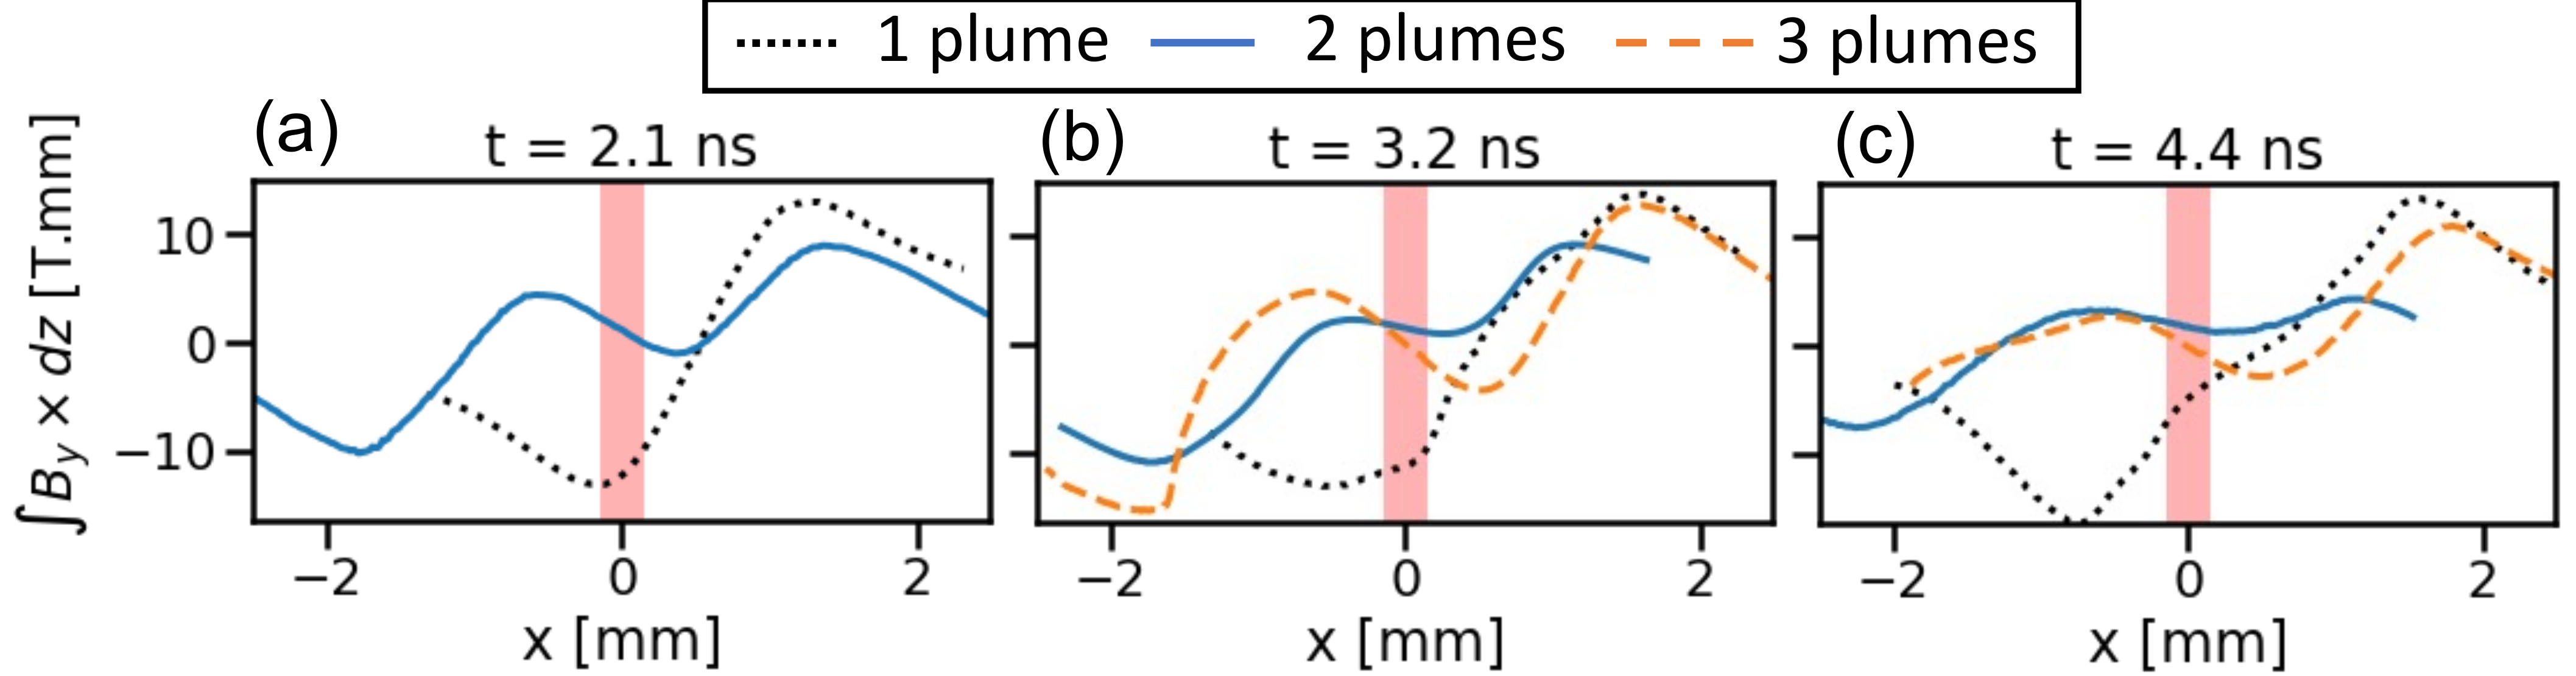
\includegraphics[width=1.0\textwidth]{problem.png}
\end{center}

$\bullet$ weaker B-field for 2-plumes \& 3-plumes : reconnection operates ! \\
$\to$ $\partial_t \phi = \partial_t \int \!\!\! \int B_y \; \D x \D z = 2.5 \pm 0.6$ T.mm$^2$.ns$^{-1}$ \\
$\to$ frow Faraday law, $\partial_t \phi = \int E \D z \sim \lambda E$ \\
$\to$ $\int B_y \; \D z = 13$ T.mm and $V_0 \sim v_A = 400 \pm 130 \times 10^3$ m.s$^{-1}$ \\

\bigskip

$\bullet$ reconnection rate $E^{\prime} = 0.48 \substack{+0.40 \\ -0.20}$ (2-plumes case) \\
$\to$ \underline{Fast reconnection} (even very fast...) \\

\end{frame}



% ____________________________________________________________________________
\begin{frame}
\frametitle{Collisional vs collisionless tearing}

$\bullet$ A current sheet is intrinsically unstable to tearing

\begin{center}
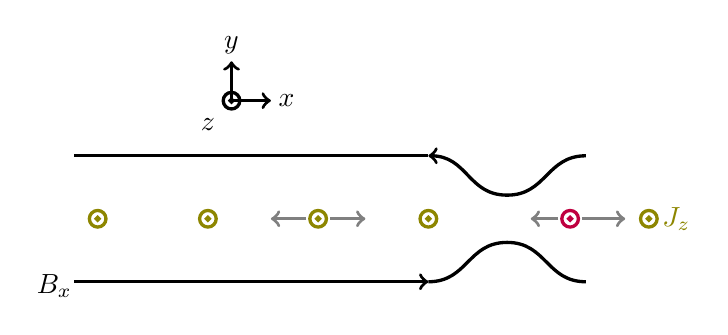
\begin{tikzpicture}[scale=0.5]

\def\dx{0.3} % diameter of the arrow
\def\l{2.8}  % mean distance between the wires
\def\arrlen{0.9}
\def\arrlenmin{0.7}
\def\arrlenmax{1.1}
\def\dl{0.8} % offset of the unaligned wire

\def\la{-9.0} % left start point of straight field line
\def\lb{-0.0} % left end point of straight field line
\def\yl{1.6} % y offset of the field line relative to 0
\def\conta{1.0} % control for outer tip of field line
\def\contb{1.0} % control for iner tip of field line
\def\lc{+2.0} % left end point of straight field line
\def\ld{+4.0} % left end point of straight field line
\def\dyl{0.6} % y location of the pinched field line


\tikzset{arrowplus/.pic = {\draw[very thick] (0, 0) circle (3pt);
                           \draw[very thick] (0, 0) circle (0.5pt); }
        }

\tikzset{arrowminus/.pic = {\draw[very thick] (0, 0) circle (3pt);
                            \draw[very thick] ( 0.0,-0.1) -- ( 0.0,+0.1);
                            \draw[very thick] (-0.1, 0.0) -- (+0.1, 0.0);}
        }


\tikzset{frame/.pic = {\draw[very thick, ->] (0.0, 0.0) -- ( 0.5, 0.0);
                       \node at ( 0.7, 0.0) {$x$};
                       \draw[very thick, ->] (0.0, 0.0) -- ( 0.0, 0.5);
                       \node at ( 0.0, 0.7) {$y$};
                       \path[very thick] (0.0 ,0.0) pic{arrowplus};
                       \node at (-0.3,-0.3) {$z$};}
        }

% wires of current
\path[very thick, olive] (0-3*\l,0) pic{arrowplus};
\path[very thick, olive] (0-2*\l,0) pic{arrowplus};
\path[very thick, olive] (0-1*\l,0) pic{arrowplus};
\path[very thick, olive] (0,0) pic{arrowplus};
\path[very thick, purple] (0+1*\l+\dl,0) pic{arrowplus};
\path[very thick, olive] (0+2*\l,0) pic{arrowplus};

% forces on the wire
\draw[very thick, gray,   ->] (0-\l-\dx, 0) -- (0-\l-\dx-\arrlen,0);
\draw[very thick, gray,   ->] (0-\l+\dx, 0) -- (0-\l+\dx+\arrlen,0);
\draw[very thick, gray,   ->] (0+\l+\dl-\dx, 0) -- (0+\l+\dl-\dx-\arrlenmin,0);
\draw[very thick, gray,   ->] (0+\l+\dl+\dx, 0) -- (0+\l+\dl+\dx+\arrlenmax,0);

% B field line
\draw[very thick, black,  ->] (\la, -\yl) -- (\lb, -\yl);
\draw[very thick, black,  - ] (\lb, -\yl)
    .. controls +(+\conta, 0) and +(-\contb, 0)
    .. (\lc, -\dyl)
    .. controls +(+\contb, 0) and +(-\conta, 0)
    .. (\ld, -\yl);

\draw[very thick, black,  - ] (\la, +\yl) -- (\lb, +\yl);
\draw[very thick, black,  <-] (\lb, +\yl)
    .. controls +(+\conta, 0) and +(-\contb, 0)
    .. (\lc, +\dyl)
    .. controls +(+\contb, 0) and +(-\conta, 0)
    .. (\ld, +\yl);

% legend
\node[olive] at ( 6.3, 0.0) {$J_z$};
\node[black] at (-9.5,-1.7) {$B_x$};

% axis
\path[very thick] (-5.0,3.0) pic{frame};

\end{tikzpicture}

\end{center}

$\bullet$ Magnetic reconnection triggers with a dissipation mechanism: \\[0.4cm]
$\to$ Coulomb collisions [\textit{Furth et al.} 1963, Phys. Fluids] \\
$\to$ Particle-wave resonant process [\textit{Coppi et al.} 1966, PRL]


\end{frame}



% ____________________________________________________________________________
\begin{frame}
\frametitle{Characteristic scales for magnetic reconnection}

$\bullet$ Collisional tearing : $\displaystyle \gamma = \frac{(\Delta^{\prime} L)^{4/5}}{\tau_R} S^{2/5}$ \\

$\to$ $S \gg 1$, $L \gg \lambda_{CS}$ collisional reconnection \& $\tau_R \ll \tau_A$ \\
$\to$ $E^{\prime} \lesssim 0.01$ for "fast" high-$S$ reconnection \\

\bigskip

$\bullet$ Collisionless tearing : $\displaystyle \gamma = \frac{1}{\sqrt{\pi}} (1 - k^2\lambda_{CS}^2) \frac{d_e^2}{\lambda_{CS}^2} \frac{v_{Te}}{\sqrt{\rho_e \lambda_{CS}}} $ \\

$\to$ $\lambda_{CS} \sim d_p$, $\rho_e \sim d_e$ so $\gamma$ is a fraction of $\Omega_p$ \\
$\to$ $E^{\prime} \sim 0.1$ for fast reconnection mediated by Hall effect \\

\bigskip

$\bullet$ Hall-MHD, hybrid-PIC \& full-PIC simulations \\
$\to$ growth on $\Omega_p t \sim 20$ [\textit{Birn et al.}, 2001, J. Geophys. Res.] \\

\bigskip

%%% $\Rightarrow$ $\lambda_{CS} \sim d_p$ over a length $L > 20 d_p$ \\[0.2cm]
$\bullet$ $\Omega_p \sim 10$ ps for $B = 10^3$ T and $d_p \sim 2 \mu$m for $n_e = 10^{28}$ m$^{-3}$ \\

\end{frame}



%%% % ____________________________________________________________________________
%%% \begin{frame}
%%% \frametitle{Big picture of 2D magnetic reconnection}
%%% 
%%% \begin{center}
%%% 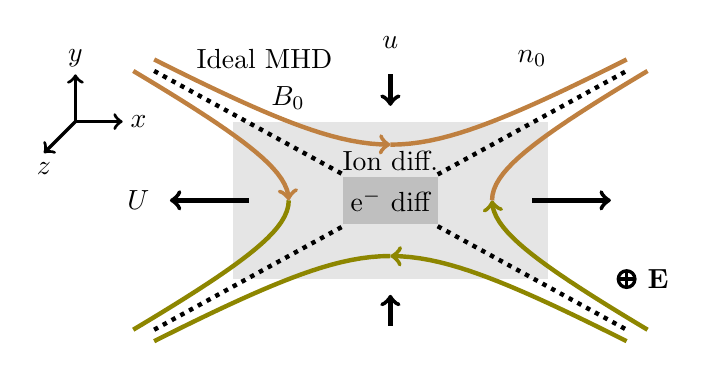
\begin{tikzpicture}[scale=1.0]

%\newcommand\XA{2} etc. and then \coordinate (A) at (\XA,\YA);

%\tikzset{declare function={f(\x)=\x;}}

\def\XIdiff{2.0}
\def\YIdiff{1.0}
\def\XEdiff{0.6}
\def\YEdiff{0.3}

\fill[gray!20] (-\XIdiff, -\YIdiff) rectangle (+\XIdiff, +\YIdiff);
\fill[gray!50] (-\XEdiff, -\YEdiff) rectangle (+\XEdiff, +\YEdiff);


\def\Xmin{-3.0}
\def\Xmax{+3.0}
\def\Xmed{+0.6}

\def\Ome{0.3}
\def\Lia{0.5}
\def\Lib{0.3}
\def\Lic{0.1}


\draw [domain=\Xmin: -\Xmed, ultra thick, dotted] plot(\x,{-sqrt(\Ome)*\x});
\draw [domain=\Xmed:  \Xmax, ultra thick, dotted] plot(\x,{-sqrt(\Ome)*\x});
\draw [domain=\Xmin: -\Xmed, ultra thick, dotted] plot(\x,{ sqrt(\Ome)*\x});
\draw [domain=\Xmed:  \Xmax, ultra thick, dotted] plot(\x,{ sqrt(\Ome)*\x});

\draw [domain=\Xmin: 0, ultra thick, draw=brown, ->] plot(\x,{sqrt( \Ome*\x*\x+\Lia)});
\draw [domain=0: \Xmax, ultra thick, draw=brown] plot(\x,{sqrt( \Ome*\x*\x+\Lia)});
%%% \draw [domain=\Xmin: \Xmax, ultra thick, draw=brown!40] plot(\x,{sqrt( \Ome*\x*\x+\Lic)});

\draw [domain=\Xmin: 0, ultra thick, draw=olive] plot(\x,{-sqrt( \Ome*\x*\x+\Lia)});
\draw [domain=0: \Xmax, ultra thick, draw=olive, <-] plot(\x,{-sqrt( \Ome*\x*\x+\Lia)});
%%% \draw [domain=\Xmin: \Xmax, ultra thick, draw=olive!40] plot(\x,{-sqrt( \Ome*\x*\x+\Lic)});

\draw [domain=\Xmin*sqrt(\Ome): 0, ultra thick, draw=olive, ->] plot({sqrt((\x*\x+\Lia)/\Ome)}, \x);
\draw [domain=0: \Xmax*sqrt(\Ome), ultra thick, draw=brown] plot({sqrt((\x*\x+\Lia)/\Ome)}, \x);
%%% \draw [domain=\Xmin*sqrt(\Ome): 0, ultra thick, draw=olive!40] plot({sqrt((\x*\x+\Lic)/\Ome)}, \x);
%%% \draw [domain=0: \Xmax*sqrt(\Ome), ultra thick, draw=brown!40] plot({sqrt((\x*\x+\Lic)/\Ome)}, \x);

\draw [domain=\Xmin*sqrt(\Ome): 0, ultra thick, draw=olive] plot({-sqrt((\x*\x+\Lia)/\Ome)}, \x);
\draw [domain=0: \Xmax*sqrt(\Ome), ultra thick, draw=brown, <-] plot({-sqrt((\x*\x+\Lia)/\Ome)}, \x);
%%% \draw [domain=\Xmin*sqrt(\Ome): 0, ultra thick, draw=olive!40] plot({-sqrt((\x*\x+\Lic)/\Ome)}, \x);
%%% \draw [domain=0: \Xmax*sqrt(\Ome), ultra thick, draw=brown!40] plot({-sqrt((\x*\x+\Lic)/\Ome)}, \x);

%%% \def\KKK{0.6}
%%% \def\XmiN{-1.6}
%%% \def\XmaX{-0.74}
%%% 
%%% \draw [domain=\XmaX: \XmiN, very thick, ->] plot(\x, {\KKK*(-\x)^(-1/\Ome)});
%%% \draw [domain=\XmaX: \XmiN, very thick, ->] plot(\x, {-\KKK*(-\x)^(-1/\Ome)});
%%% \draw [domain=-\XmaX: -\XmiN, very thick, ->] plot(\x, {\KKK*(\x)^(-1/\Ome)});
%%% \draw [domain=-\XmaX: -\XmiN, very thick, ->] plot(\x, {-\KKK*(\x)^(-1/\Ome)});


%%% \def\Xa{0.89}
%%% \def\Xb{1.35}
%%% 
%%% \filldraw[fill=black!60] (\Xa, {\KKK*(\Xa)^(-1/\Ome)}) circle (2pt);
%%% \filldraw[fill=black!60] (\Xb, {\KKK*(\Xb)^(-1/\Ome)}) circle (2pt);
%%% \filldraw[fill=black!60] (-\Xa, {\KKK*(\Xa)^(-1/\Ome)}) circle (2pt);
%%% \filldraw[fill=black!60] (-\Xb, {\KKK*(\Xb)^(-1/\Ome)}) circle (2pt);
%%% 
%%% \filldraw[fill=black!20] (\Xa, -{\KKK*(\Xa)^(-1/\Ome)}) circle (2pt);
%%% \filldraw[fill=black!20] (\Xb, -{\KKK*(\Xb)^(-1/\Ome)}) circle (2pt);
%%% \filldraw[fill=black!20] (-\Xa, -{\KKK*(\Xa)^(-1/\Ome)}) circle (2pt);
%%% \filldraw[fill=black!20] (-\Xb, -{\KKK*(\Xb)^(-1/\Ome)}) circle (2pt);



\draw[very thick] ( 3.0,-1.0) circle (3pt);
\draw[very thick] ( 2.9,-1.0) -- ( 3.1,-1.0);
\draw[very thick] ( 3.0,-1.1) -- ( 3.0,-0.9);
\node at ( 3.4,-1.0) {$\mathbf E$};

\draw[ultra thick, <-] (-2.8, 0) -- (-1.8, 0);
\draw[ultra thick, ->] (1.8, 0) -- (2.8, 0);
\node at (-3.2, 0.0) {$U$};

\draw[ultra thick, ->] ( 0.0, 1.6) -- ( 0.0, 1.2);
\draw[ultra thick, <-] ( 0.0,-1.2) -- ( 0.0,-1.6);
\node at ( 0.0, 2.0) {$u$};

\node at (-1.3, 1.3) {$B_0$};
\node at ( 1.8, 1.8) {$n_0$};

\node at (-1.6, 1.8) {Ideal MHD};
\node at (-0.0, 0.5) {Ion diff.};
\node at (-0.0, 0.0) {e$^-$ diff};


\draw[very thick, ->] (-4.0, 1.0) -- (-3.4, 1.0);
\node at (-3.2, 1.0) {$x$};
\draw[very thick, ->] (-4.0, 1.0) -- (-4.0, 1.6);
\node at (-4.0, 1.8) {$y$};
\draw[very thick, ->] (-4.0, 1.0) -- (-4.4, 0.6);
\node at (-4.4, 0.4) {$z$};


\end{tikzpicture}

%%% \end{center}
%%% 
%%% $\bullet$ Ohm's law : $\mathbf E = - \mathbf V \times \mathbf B - \frac{1}{en} [\mathbf j \times \mathbf B - \boldsymbol{\nabla} . \; \mathbf p_e] + \eta \mathbf j - \eta^{\prime} \Delta \mathbf j + m_e \D _t \mathbf j$ \\[0.4cm]
%%% $\to$ Ideal term in the MHD region \\
%%% $\to$ Hall term in the Ion diffusion region (control $E^{\prime}$) \\
%%% $\to$ Agyrotropic pressure term in the electron region (control $J_z$) \\
%%% 
%%% \end{frame}



% ____________________________________________________________________________
\begin{frame}
\frametitle{Hall term in the ion diffusion region}

\begin{center}
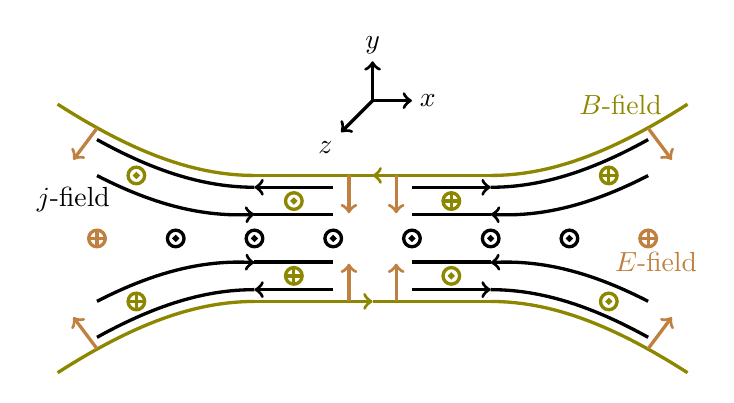
\begin{tikzpicture}[scale=0.5]

\def\shift{+3.0}
\def\dyb{1.6}
\def\eta{6.0}
\def\aa{1.0}
\def\bb{1.0}
\def\xmax{+8.}

\def\xbza{2.0}
\def\ybza{0.95}
\def\xbzb{6.0}
\def\ybzb{1.6}

\def\dyja{1.3}
\def\dyjb{0.6}
\def\zeta{6.0}
\def\shiftja{+3.0}
\def\shiftjb{+3.4}
\def\xmaxj{+7.}
\def\xminj{+1.}

\def\xea{+7.0}
\def\yea{+2.8}
\def\xeb{+7.6}
\def\yeb{+2.0}

\def\xec{0.2*\shift}
\def\yec{0.4*\dyb}

\tikzset{declare function={bline_tl(\x)=+\dyb-\eta*\bb+\bb*sqrt(\eta*\eta+((-\x-\shift)/\aa)^2);}}
\tikzset{declare function={bline_tr(\x)=+\dyb-\eta*\bb+\bb*sqrt(\eta*\eta+((+\x-\shift)/\aa)^2);}}
\tikzset{declare function={bline_bl(\x)=-\dyb+\eta*\bb-\bb*sqrt(\eta*\eta+((-\x-\shift)/\aa)^2);}}
\tikzset{declare function={bline_br(\x)=-\dyb+\eta*\bb-\bb*sqrt(\eta*\eta+((+\x-\shift)/\aa)^2);}}

\tikzset{arrowplus/.pic = {\draw[very thick] (0, 0) circle (3pt);
                           \draw[very thick] (0, 0) circle (0.5pt); }
        }

\tikzset{arrowminus/.pic = {\draw[very thick] (0, 0) circle (3pt);
                            \draw[very thick] ( 0.0,-0.1) -- ( 0.0,+0.1);
                            \draw[very thick] (-0.1, 0.0) -- (+0.1, 0.0);}
        }

\tikzset{declare function={jlinea_tl(\x)=+\dyja-\zeta*\bb+\bb*sqrt(\zeta*\eta+((-\x-\shiftja)/\aa)^2);}}
\tikzset{declare function={jlineb_tl(\x)=+\dyjb-\zeta*\bb+\bb*sqrt(\zeta*\eta+((-\x-\shiftjb)/\aa)^2);}}
\tikzset{declare function={jlinea_tr(\x)=+\dyja-\zeta*\bb+\bb*sqrt(\zeta*\eta+((+\x-\shiftja)/\aa)^2);}}
\tikzset{declare function={jlineb_tr(\x)=+\dyjb-\zeta*\bb+\bb*sqrt(\zeta*\eta+((+\x-\shiftjb)/\aa)^2);}}
\tikzset{declare function={jlinea_bl(\x)=-\dyja+\zeta*\bb-\bb*sqrt(\zeta*\eta+((-\x-\shiftja)/\aa)^2);}}
\tikzset{declare function={jlineb_bl(\x)=-\dyjb+\zeta*\bb-\bb*sqrt(\zeta*\eta+((-\x-\shiftjb)/\aa)^2);}}
\tikzset{declare function={jlinea_br(\x)=-\dyja+\zeta*\bb-\bb*sqrt(\zeta*\eta+((+\x-\shiftja)/\aa)^2);}}
\tikzset{declare function={jlineb_br(\x)=-\dyjb+\zeta*\bb-\bb*sqrt(\zeta*\eta+((+\x-\shiftjb)/\aa)^2);}}

\tikzset{frame/.pic = {\draw[very thick, ->] (0.0, 0.0) -- ( 0.5, 0.0);
                       \node at ( 0.7, 0.0) {$x$};
                       \draw[very thick, ->] (0.0, 0.0) -- ( 0.0, 0.5);
                       \node at ( 0.0, 0.7) {$y$};
                       \draw[very thick, ->] (0.0, 0.0) -- (-0.4,-0.4);
                       \node at (-0.6,-0.6) {$z$};}
        }

%B field in xy plane
\draw[very thick, olive,   -] (-\shift, \dyb) -- (0, \dyb);
\draw [domain=-\xmax:-\shift, very thick, olive,  -] plot(\x, {bline_tl(\x)});

\draw[very thick, olive,  ->] (\shift, \dyb) -- (0, \dyb);
\draw [domain=\shift:\xmax, very thick, olive,  -] plot(\x, {bline_tr(\x)});

\draw[very thick, olive,  ->] (-\shift, -\dyb) -- (0, -\dyb);
\draw [domain=-\xmax:-\shift, very thick, olive,  -] plot(\x, {bline_bl(\x)});

\draw[very thick, olive,   -] (\shift, -\dyb) -- (0, -\dyb);
\draw [domain=\shift:\xmax, very thick, olive,  -] plot(\x, {bline_br(\x)});

%B field along z
\path[very thick, olive] (-\xbza,+\ybza) pic{arrowplus};
\path[very thick, olive] (+\xbza,+\ybza) pic{arrowminus};
\path[very thick, olive] (-\xbza,-\ybza) pic{arrowminus};
\path[very thick, olive] (+\xbza,-\ybza) pic{arrowplus};

\path[very thick, olive] (-\xbzb,+\ybzb) pic{arrowplus};
\path[very thick, olive] (+\xbzb,+\ybzb) pic{arrowminus};
\path[very thick, olive] (-\xbzb,-\ybzb) pic{arrowminus};
\path[very thick, olive] (+\xbzb,-\ybzb) pic{arrowplus};

%J field in xy plane
\draw [domain=-\xmaxj:-\shift, very thick, black,  -] plot(\x, {jlinea_tl(\x)});
\draw [very thick, black,  ->] (-\xminj,  \dyja) -- (-\shift, \dyja);
\draw [domain=-\shift:-\xmaxj, very thick, black, <-] plot(\x, {jlineb_tl(\x)});
\draw [very thick, black,   -] (-\shift,  \dyjb) -- (-\xminj,  \dyjb);

\draw [domain= \xmaxj: \shift, very thick, black,  -] plot(\x, {jlinea_tr(\x)});
\draw [very thick, black,  ->] ( \xminj,  \dyja) -- ( \shift, \dyja);
\draw [domain= \shift: \xmaxj, very thick, black, <-] plot(\x, {jlineb_tr(\x)});
\draw [very thick, black,   -] ( \shift,  \dyjb) -- ( \xminj,  \dyjb);

\draw [domain=-\xmaxj:-\shift, very thick, black,  -] plot(\x, {jlinea_bl(\x)});
\draw [very thick, black,  ->] (-\xminj,-\dyja) -- (-\shift, -\dyja);
\draw [domain=-\shift:-\xmaxj, very thick, black, <-] plot(\x, {jlineb_bl(\x)});
\draw [very thick, black,   -] (-\shift, -\dyjb) -- (-\xminj, -\dyjb);

\draw [domain= \xmaxj: \shift, very thick, black,  -] plot(\x, {jlinea_br(\x)});
\draw [very thick, black,  ->] ( \xminj, -\dyja) -- ( \shift, -\dyja);
\draw [domain= \shift: \xmaxj, very thick, black, <-] plot(\x, {jlineb_br(\x)});
\draw [very thick, black,   -] ( \shift, -\dyjb) -- ( \xminj, -\dyjb);

%J field along z
\path[very thick, black] (-5, 0) pic{arrowplus};
\path[very thick, black] (-3, 0) pic{arrowplus};
\path[very thick, black] (-1, 0) pic{arrowplus};
\path[very thick, black] ( 1, 0) pic{arrowplus};
\path[very thick, black] ( 3, 0) pic{arrowplus};
\path[very thick, black] ( 5, 0) pic{arrowplus};

%E field in the XY plane
\draw [very thick, brown, ->] (-\xea, \yea) -- (-\xeb, \yeb);
\draw [very thick, brown, ->] ( \xea, \yea) -- ( \xeb, \yeb);
\draw [very thick, brown, ->] (-\xea,-\yea) -- (-\xeb,-\yeb);
\draw [very thick, brown, ->] ( \xea,-\yea) -- ( \xeb,-\yeb);

\draw [very thick, brown, ->] (-\xec, \dyb) -- (-\xec, \yec);
\draw [very thick, brown, ->] ( \xec, \dyb) -- ( \xec, \yec);
\draw [very thick, brown, ->] (-\xec,-\dyb) -- (-\xec,-\yec);
\draw [very thick, brown, ->] ( \xec,-\dyb) -- ( \xec,-\yec);

%J field along z
\path[very thick, brown] (-7, 0) pic{arrowminus};
\path[very thick, brown] ( 7, 0) pic{arrowminus};

\node[olive] at ( 6.3, 3.4) {$B$-field};
\node[black] at (-7.6, 1.0) {$j$-field};
\node[brown] at ( 7.2,-0.6) {$E$-field};

% axis
\path[very thick] (0.0,3.5) pic{frame};

\end{tikzpicture}

\end{center}

$\bullet$ (Hall) $E_{XY}$ electric field associated to $J_Z$ and $B_{XY}$ \\[0.3cm]
$\bullet$ $J_Z$ grows at the tip of each loops when colliding\\
$\to$ quadrupolar $B_Z$ grows because $E_{XY}$ is no more curl-free\\[0.3cm]
$\bullet$ $J_{XY}$ associated to this out-of-plane magnetic field\\
$\to$ carried by electrons because protons are demagnetized

\end{frame}



% ____________________________________________________________________________
\begin{frame}
\frametitle{Relativistic magnetic reconnection ($\sigma > 1$)}

Investigated by [\textit{Raymond et al.}, 2018, PRL] \\
$\to$ 2 J \& 40 fs w. \textsc{hercules} \& 500 J \& 20 ps w. \textsc{omega-ep} \\
$\to$ quadrupolar Hall-like B-field using \textsc{osiris} 3D full-PIC code \\

\smallskip

$\bullet$ Create $B \sim 10^4$ T in a $e^-$ coronae expanding at $\sim c$ \\

$\to$ X-ray imaging of  $e^-$ current sheet (resolved in space and time) \\
$\to$ Multi-channel spectrometer : Non-thermal electron populations \\

\begin{center}
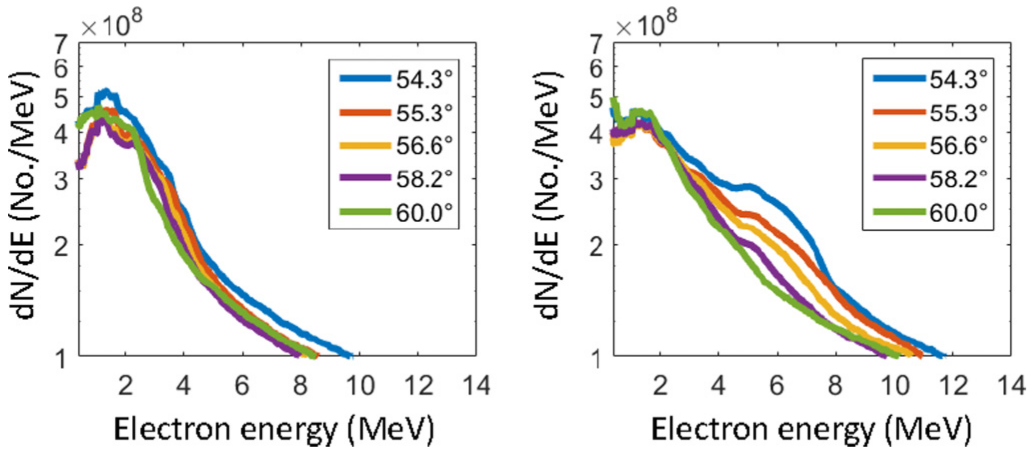
\includegraphics[width=0.8\textwidth]{raymond2018.png}
\end{center}

$\bullet$ Heating of the current-sheet $e^-$ by reconnection

\end{frame}



% ____________________________________________________________________________
\begin{frame}
\frametitle{Relativistic magnetic reconnection ($\sigma > 1$)}

Also investigated by [\textit{Palmer et al.}, 2019, PoP] \\
$\to$ using 220 J \& 9.6 ps w. \textsc{vulcan} \& proton probing (by TNSA) \\

\begin{center}
\begin{tabular}{lll}
$p^+$ RCF \hspace{2.0cm} & $p^+$ dose \hspace{2.0cm} & $B$-field \\
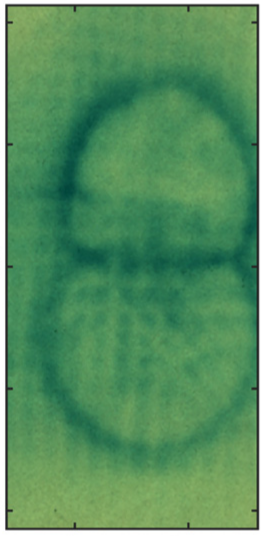
\includegraphics[width=0.25\textwidth]{palmer2019_a.png} &
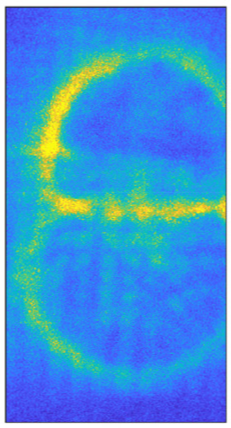
\includegraphics[width=0.28\textwidth]{palmer2019_b.png} &
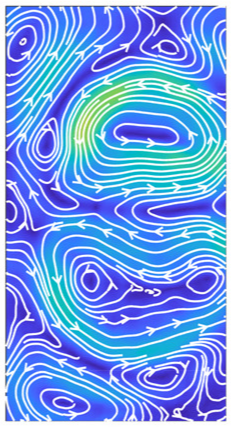
\includegraphics[width=0.28\textwidth]{palmer2019_c.png} \\
\end{tabular}
\end{center}

$\to$ In the frame of eMHD [\textit{Gordeev et al.,}, 1994, Phys. Rep.] ?

\end{frame}



% ____________________________________________________________________________
\begin{frame}
\frametitle{Reconnection in electron-positron (pair) plasma}

$\bullet$ Important in extra-galactic jets and pulsar (striped) winds \\
$\to$ Need to derive a relativistic Ohm's law to get $E^{\prime}$ \\

\bigskip

$\bullet$ No more Hall term in an electron-positron plasma\\
$\to$ "single" diffusion region [\textit{Bessho \& Bhattacharjee} 2005, PRL] \\
$\to$ the reconnection rate is still $E^{\prime} \sim 0.1$ \\
$\to$ dynamics on the electron scales... well suited for ps lasers \\

\bigskip

$\bullet$ Produced in the Lab [\textit{Greaves \& Surko}, 1995 PRL] :\\
$\to$ positron created by $\beta$-radiactive source ($^{22}$Na) \& Penning traps \\

\bigskip

$\bullet$ May we envision such an experiment on Appollon ?

\end{frame}



% ____________________________________________________________________________
\begin{frame}
\frametitle{Concluding remarks}

$\bullet$ Competiting effects of Biermann-battery and reconnection \\
$\to$ B-field created by Biermann-battery : source term \\
$\to$ B-field is then reconnected : loss term \\[0.6cm]

$\bullet$ We already measured fast reconnection : $E^{\prime} > 0.48$ \\
$\to$ first measure (of a lower value) of a reconnection rate \\[0.6cm]

$\bullet$ For long pulse lasers, one can play with target geometry \\
$\to$ guide-field, initial quadrupolar B-field \\[0.6cm]

$\bullet$ For short-pulse lasers, scales need to lowered \\
$\to$ enough time to trigger reconnection (strongly driven) ? \\
$\to$ pair plasma of interest in compact objects... \\

\end{frame}













% ____________________________________________________________________________
\begin{frame}
\frametitle{}

{\usebeamercolor[fg]{title} {\LARGE Additional material,}}

\end{frame}



% ____________________________________________________________________________
\begin{frame}
\frametitle{Hybrid-PIC simulation using \texttt{heckle}}

$\bullet$ Creation of a "Hall" quadrupolar B-field\\

\begin{center}
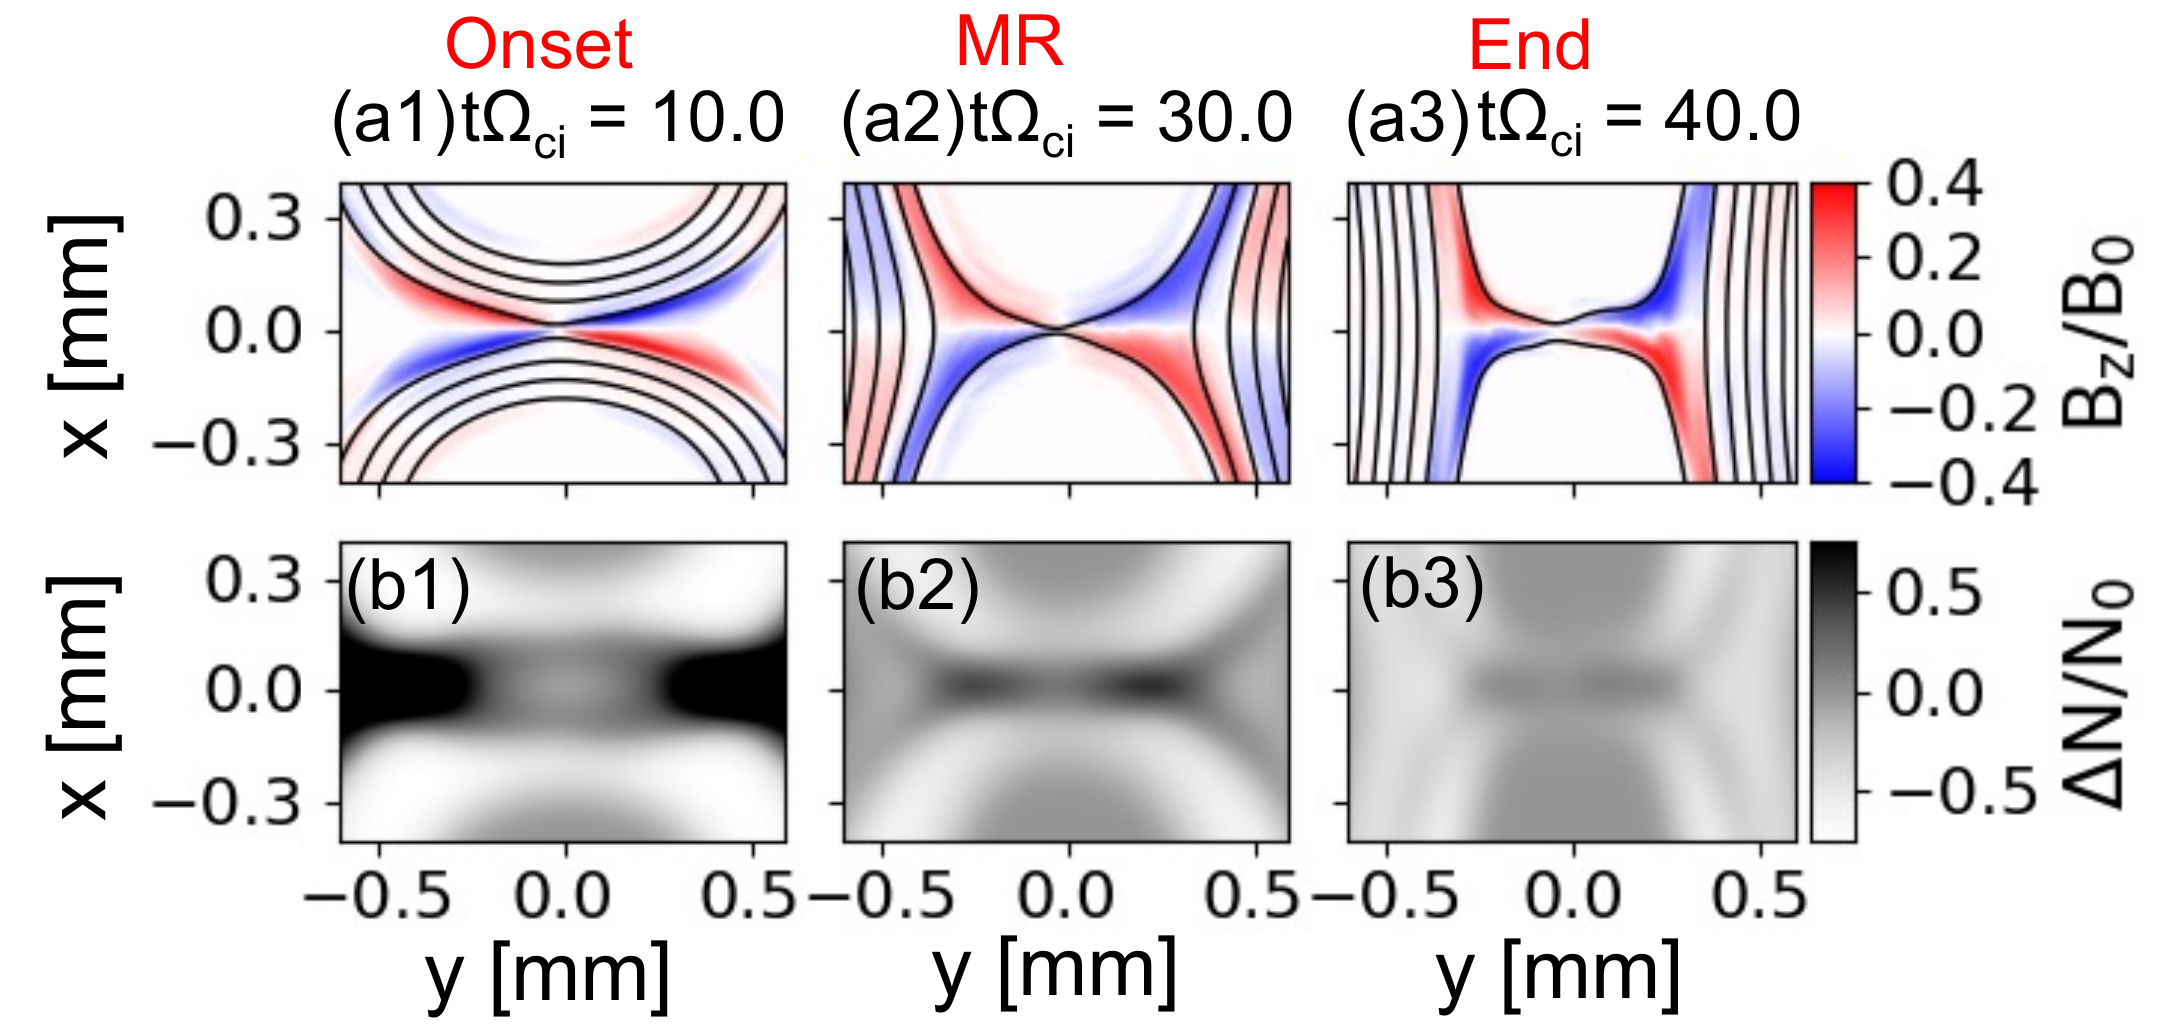
\includegraphics[width=1.0\textwidth]{heckle.png}
\end{center}

$\to$ the "mouth" opens just before the onset \\
$\to$ then closes during reconnection \\
$\to$ and disappears when there is no more B-field \\

\end{frame}



% ____________________________________________________________________________
\begin{frame}
\frametitle{DP1 images}

\begin{center}
\begin{tabular}{ccc}
shot 1 & shot 3 & shot 4 \hspace{2.0cm}\\
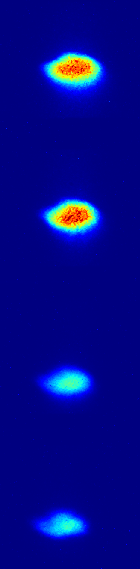
\includegraphics[width=0.14\textwidth]{dp1_1.png} &
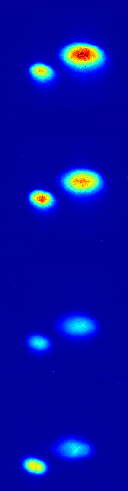
\includegraphics[width=0.14\textwidth]{dp1_2.png} &
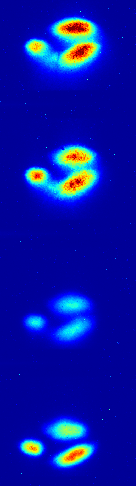
\includegraphics[width=0.14\textwidth]{dp1_3.png} \\
\end{tabular}
\end{center}

\end{frame}



% ____________________________________________________________________________
\begin{frame}
\frametitle{DMX spectra}

\begin{center}
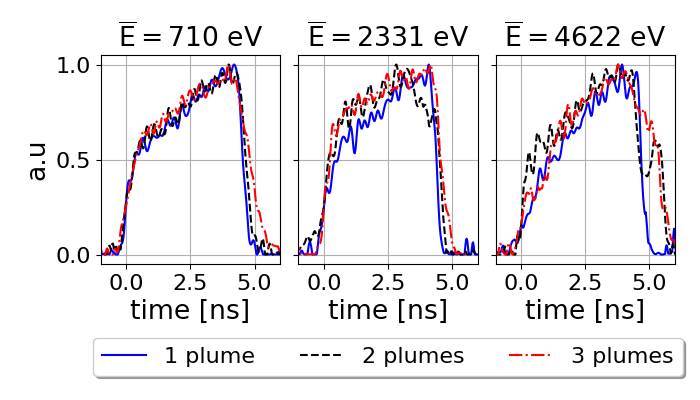
\includegraphics[width=0.8\textwidth]{fig_DMX.png}
\end{center}

$\to$ unfortunately, no clear insights from these spectra...

\end{frame}



% ____________________________________________________________________________
\begin{frame}
\frametitle{Numerical reconnection rate with \texttt{heckle}}

$\bullet$ We then "measured" $E^{\prime}$ at the saddle point \& $U_y$ \\

\begin{center}
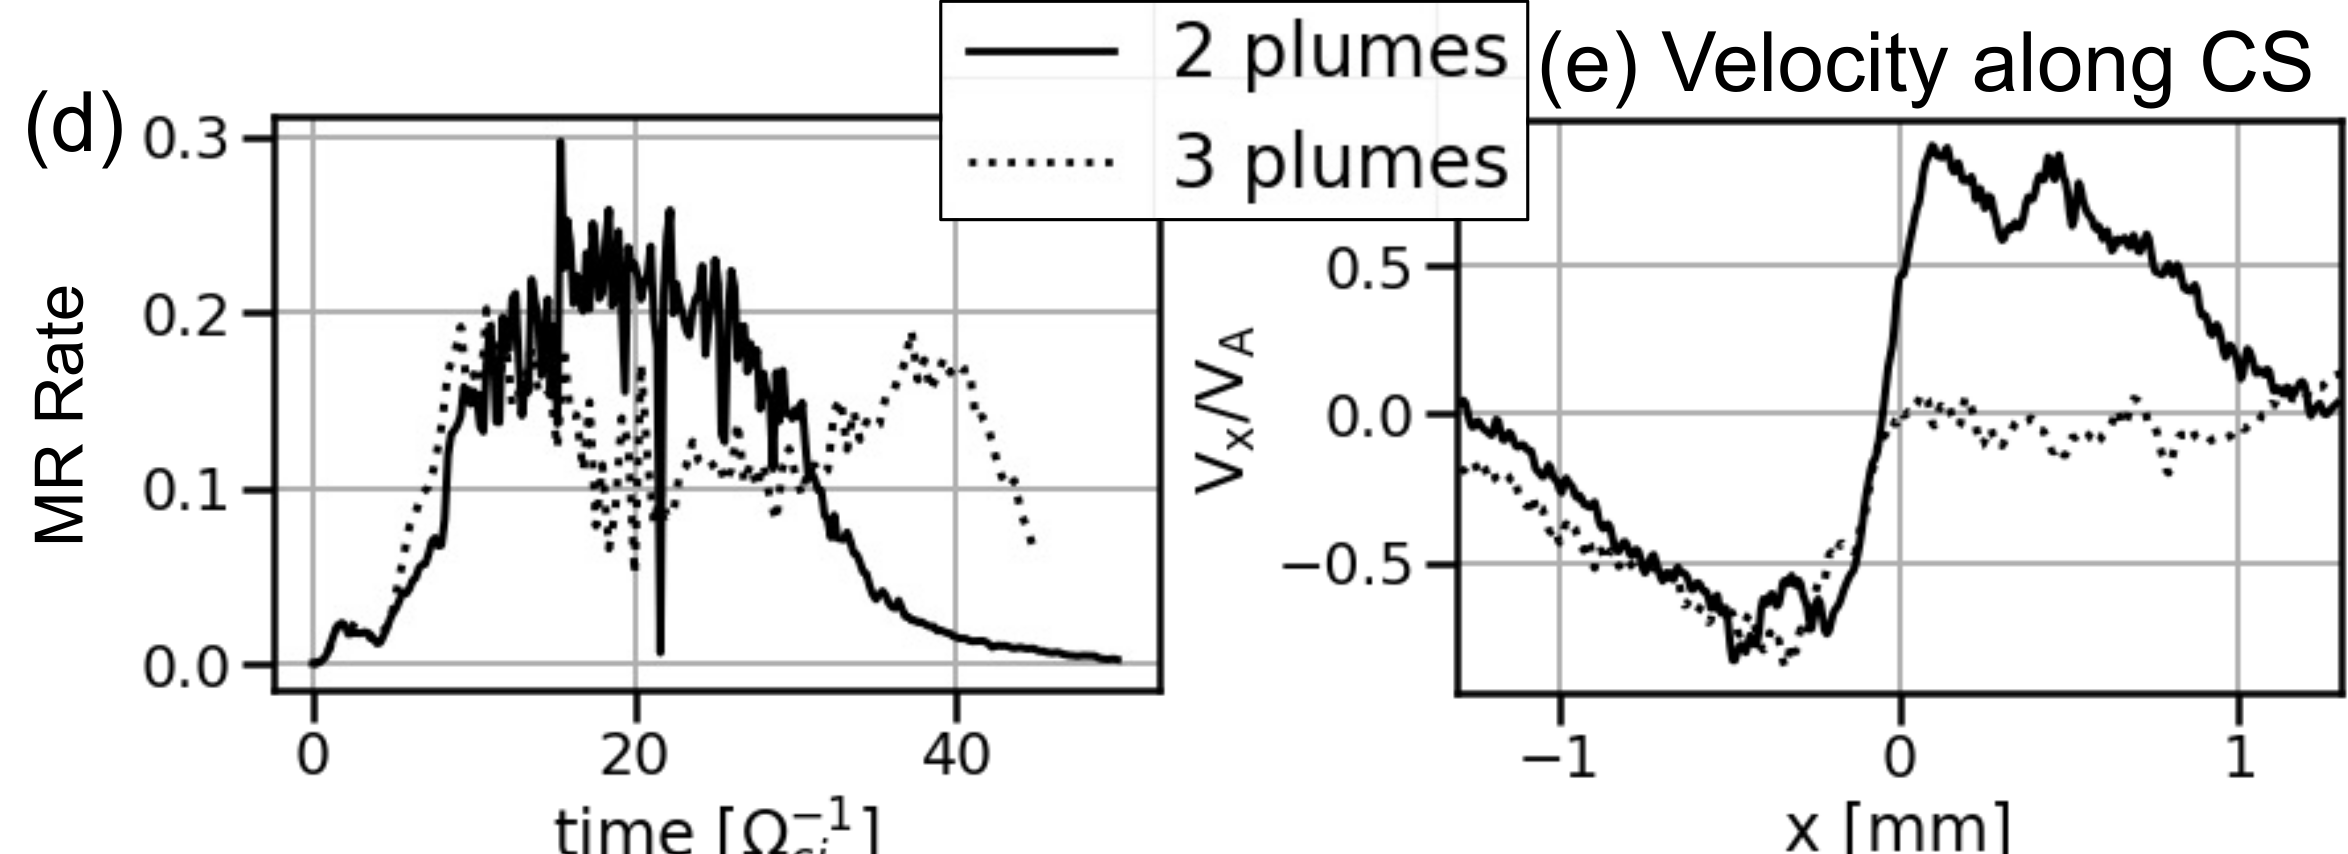
\includegraphics[width=1.0\textwidth]{recrate.png}
\end{center}

$\bullet$ The reconnection rate ($E^{\prime} \sim 0.2$) is clearly fast \\
$\to$ smaller reconnection rate with 2 plumes \\
$\to$ the outflow velocity is clearly inhibited by the closed structure \\

\end{frame}



\end{document}
